\section{CAIDA \& Atlas Analyses}\label{sec:caida_results}\todo{Proofread and trim down phrasing}

Once data \etl was complete, analysis in earnest was possible. The following sections describe analysis of the \caida and \ripe Atlas data in a natural progression from analysis of data quality, to basic connectivity analysis, and finally to geographic plotting and \gis tooling.

\subsection{Data Quality}

To gain a better understanding of the quality of the data, a series of charts were made using kernel density estimation with a Gaussian kernel. These charts should be read in a similar fashion to probability distribution functions.

\begin{figure}[H]
    \centering
    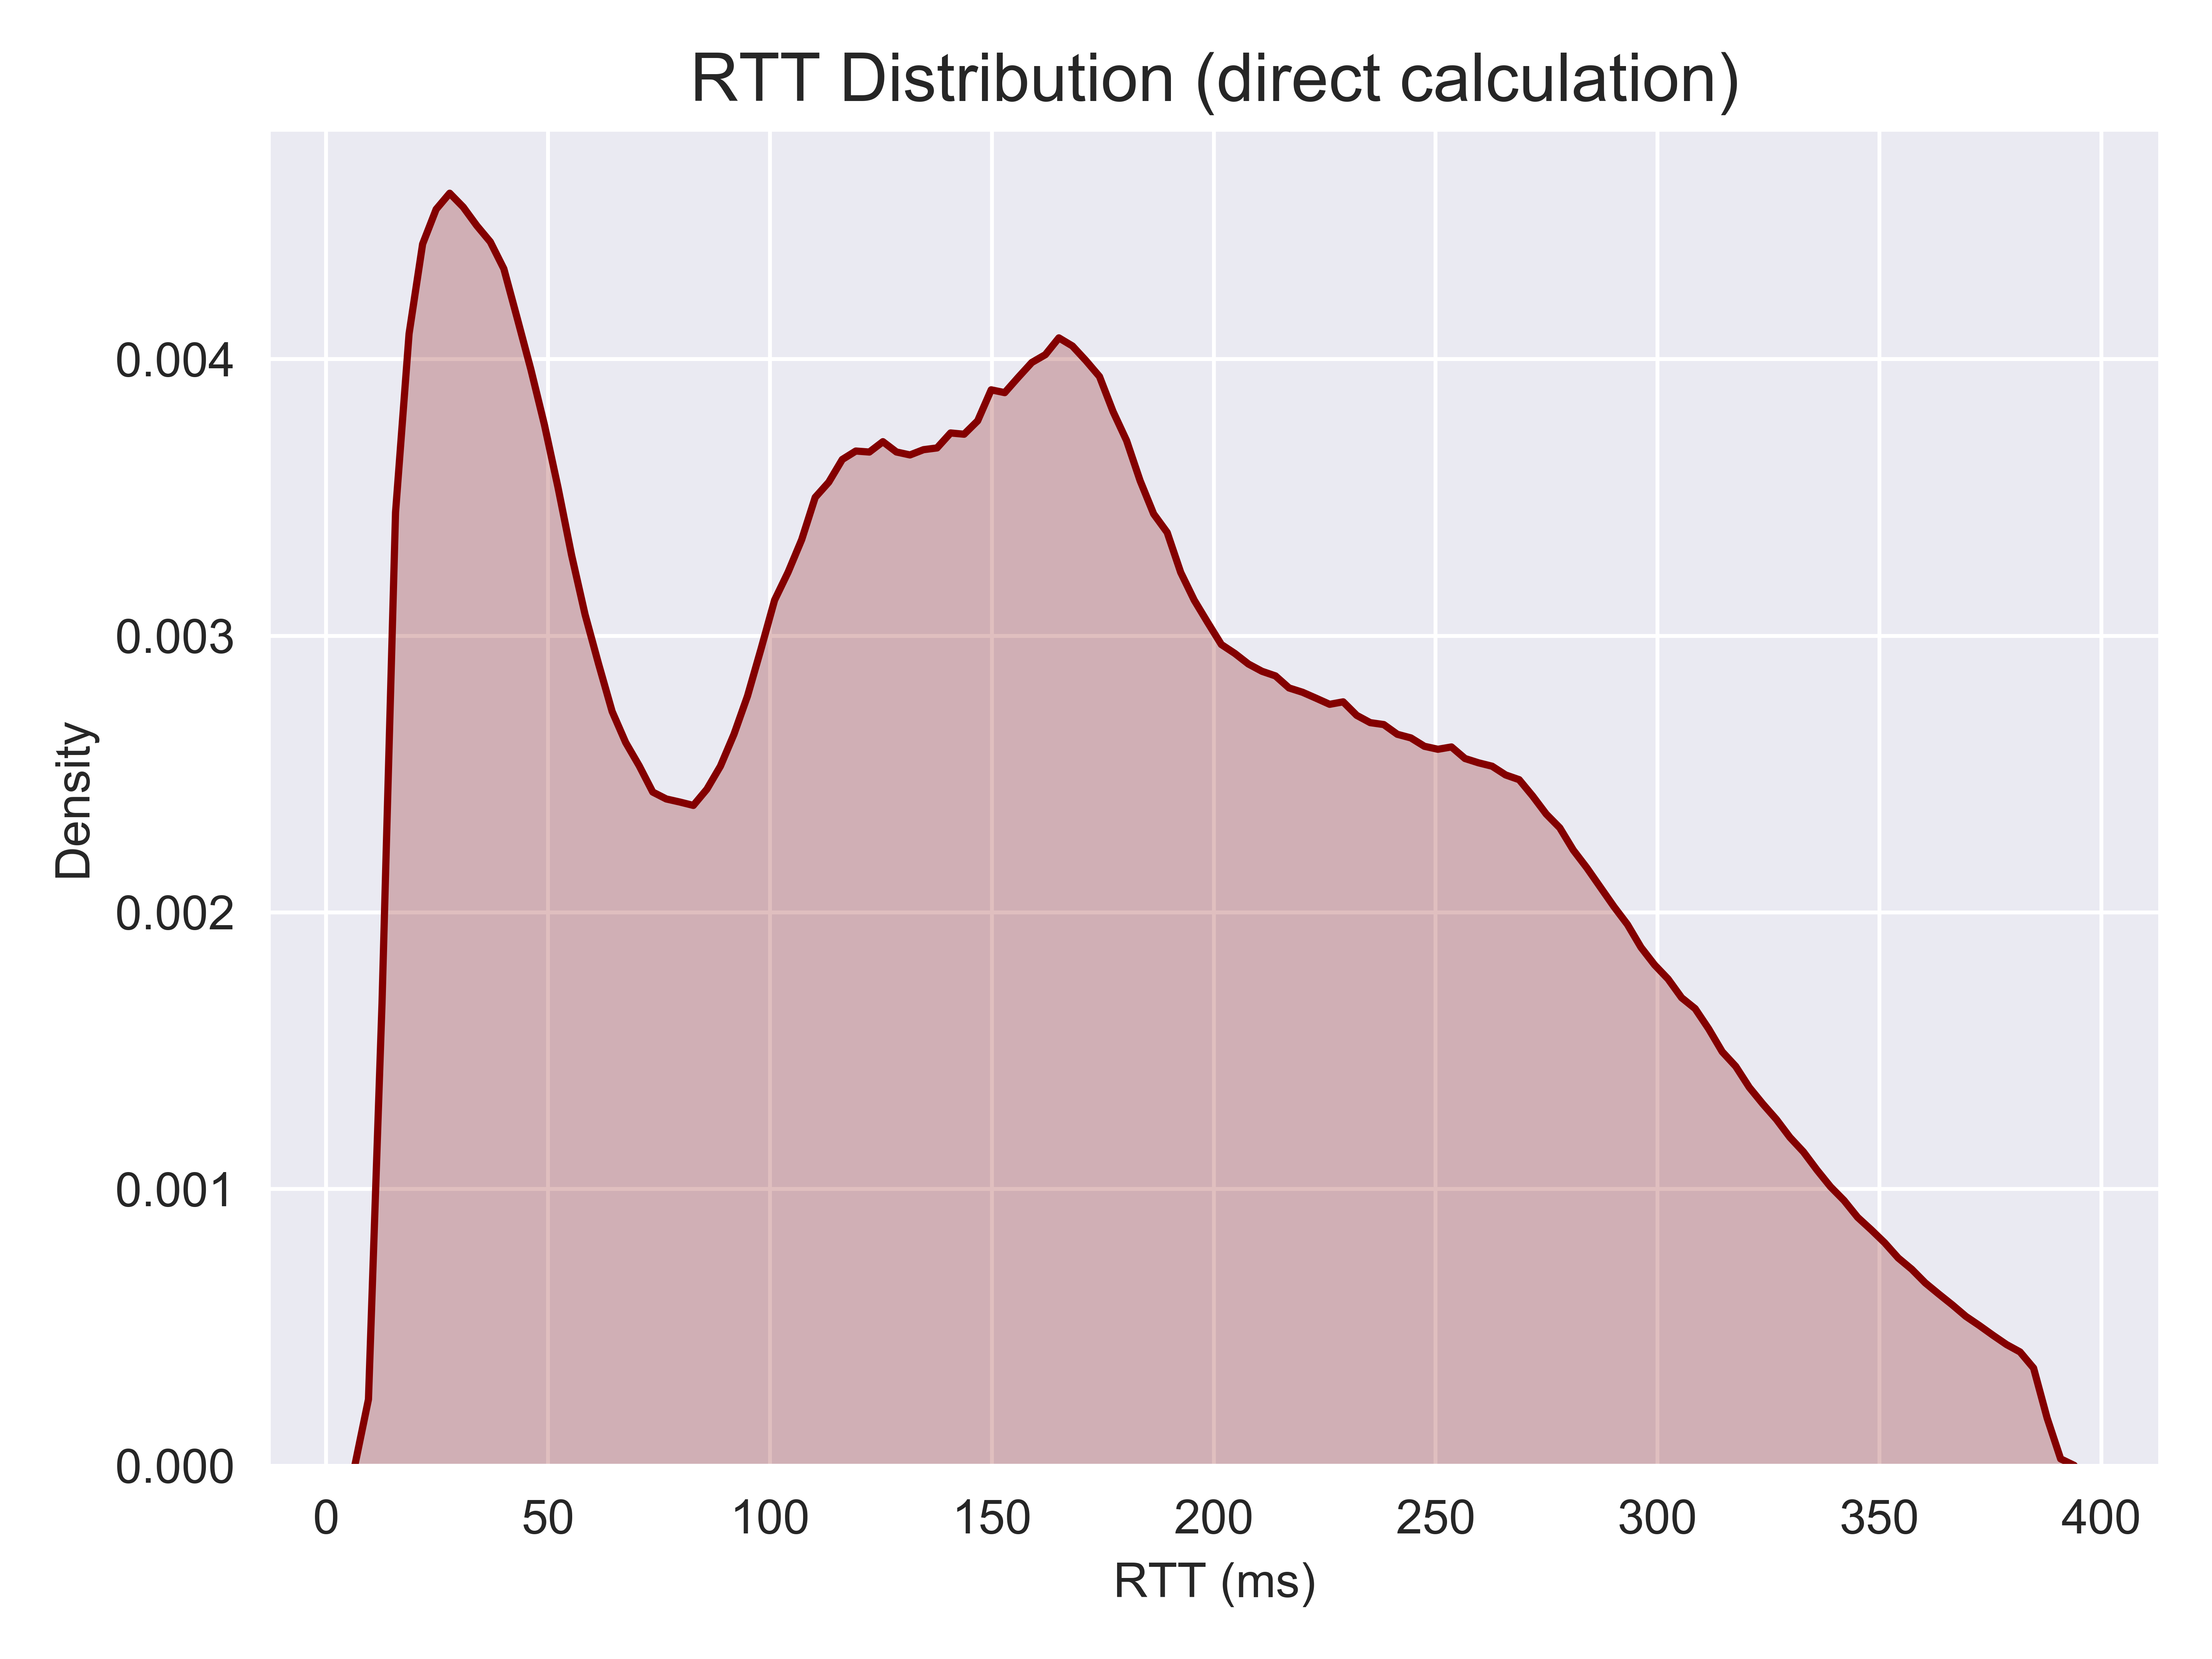
\includegraphics[width=0.75\textwidth]{caida/rtt_distribution.png}
    \caption{Distribution of RTT between IP pairs, direct ping calculation}
    \label{fig:caida_rtt_distribution}
\end{figure}\todo{Fix chart placement}

The most immediately useful distribution is that of the \rtt between \ip pairs, shown for direct-calculated \rtts in \autoref{fig:caida_rtt_distribution}. The distribution appears weakly bimodal, which we hypothesize is due to the global nature of \ripe Atlas and \caida's individual measurement networks. The leftmost peak would correspond to measurements to a device that shares a land mass with the device performing the \gls{traceroute}, while the right peak would correspond to a combination of devices on a different land mass and devices with lower-performing connections. \autoref{fig:caida_distance_distribution} appears to confirm this hypothesis, since it too is similarly bimodal.

\begin{figure}[H]
    \centering
    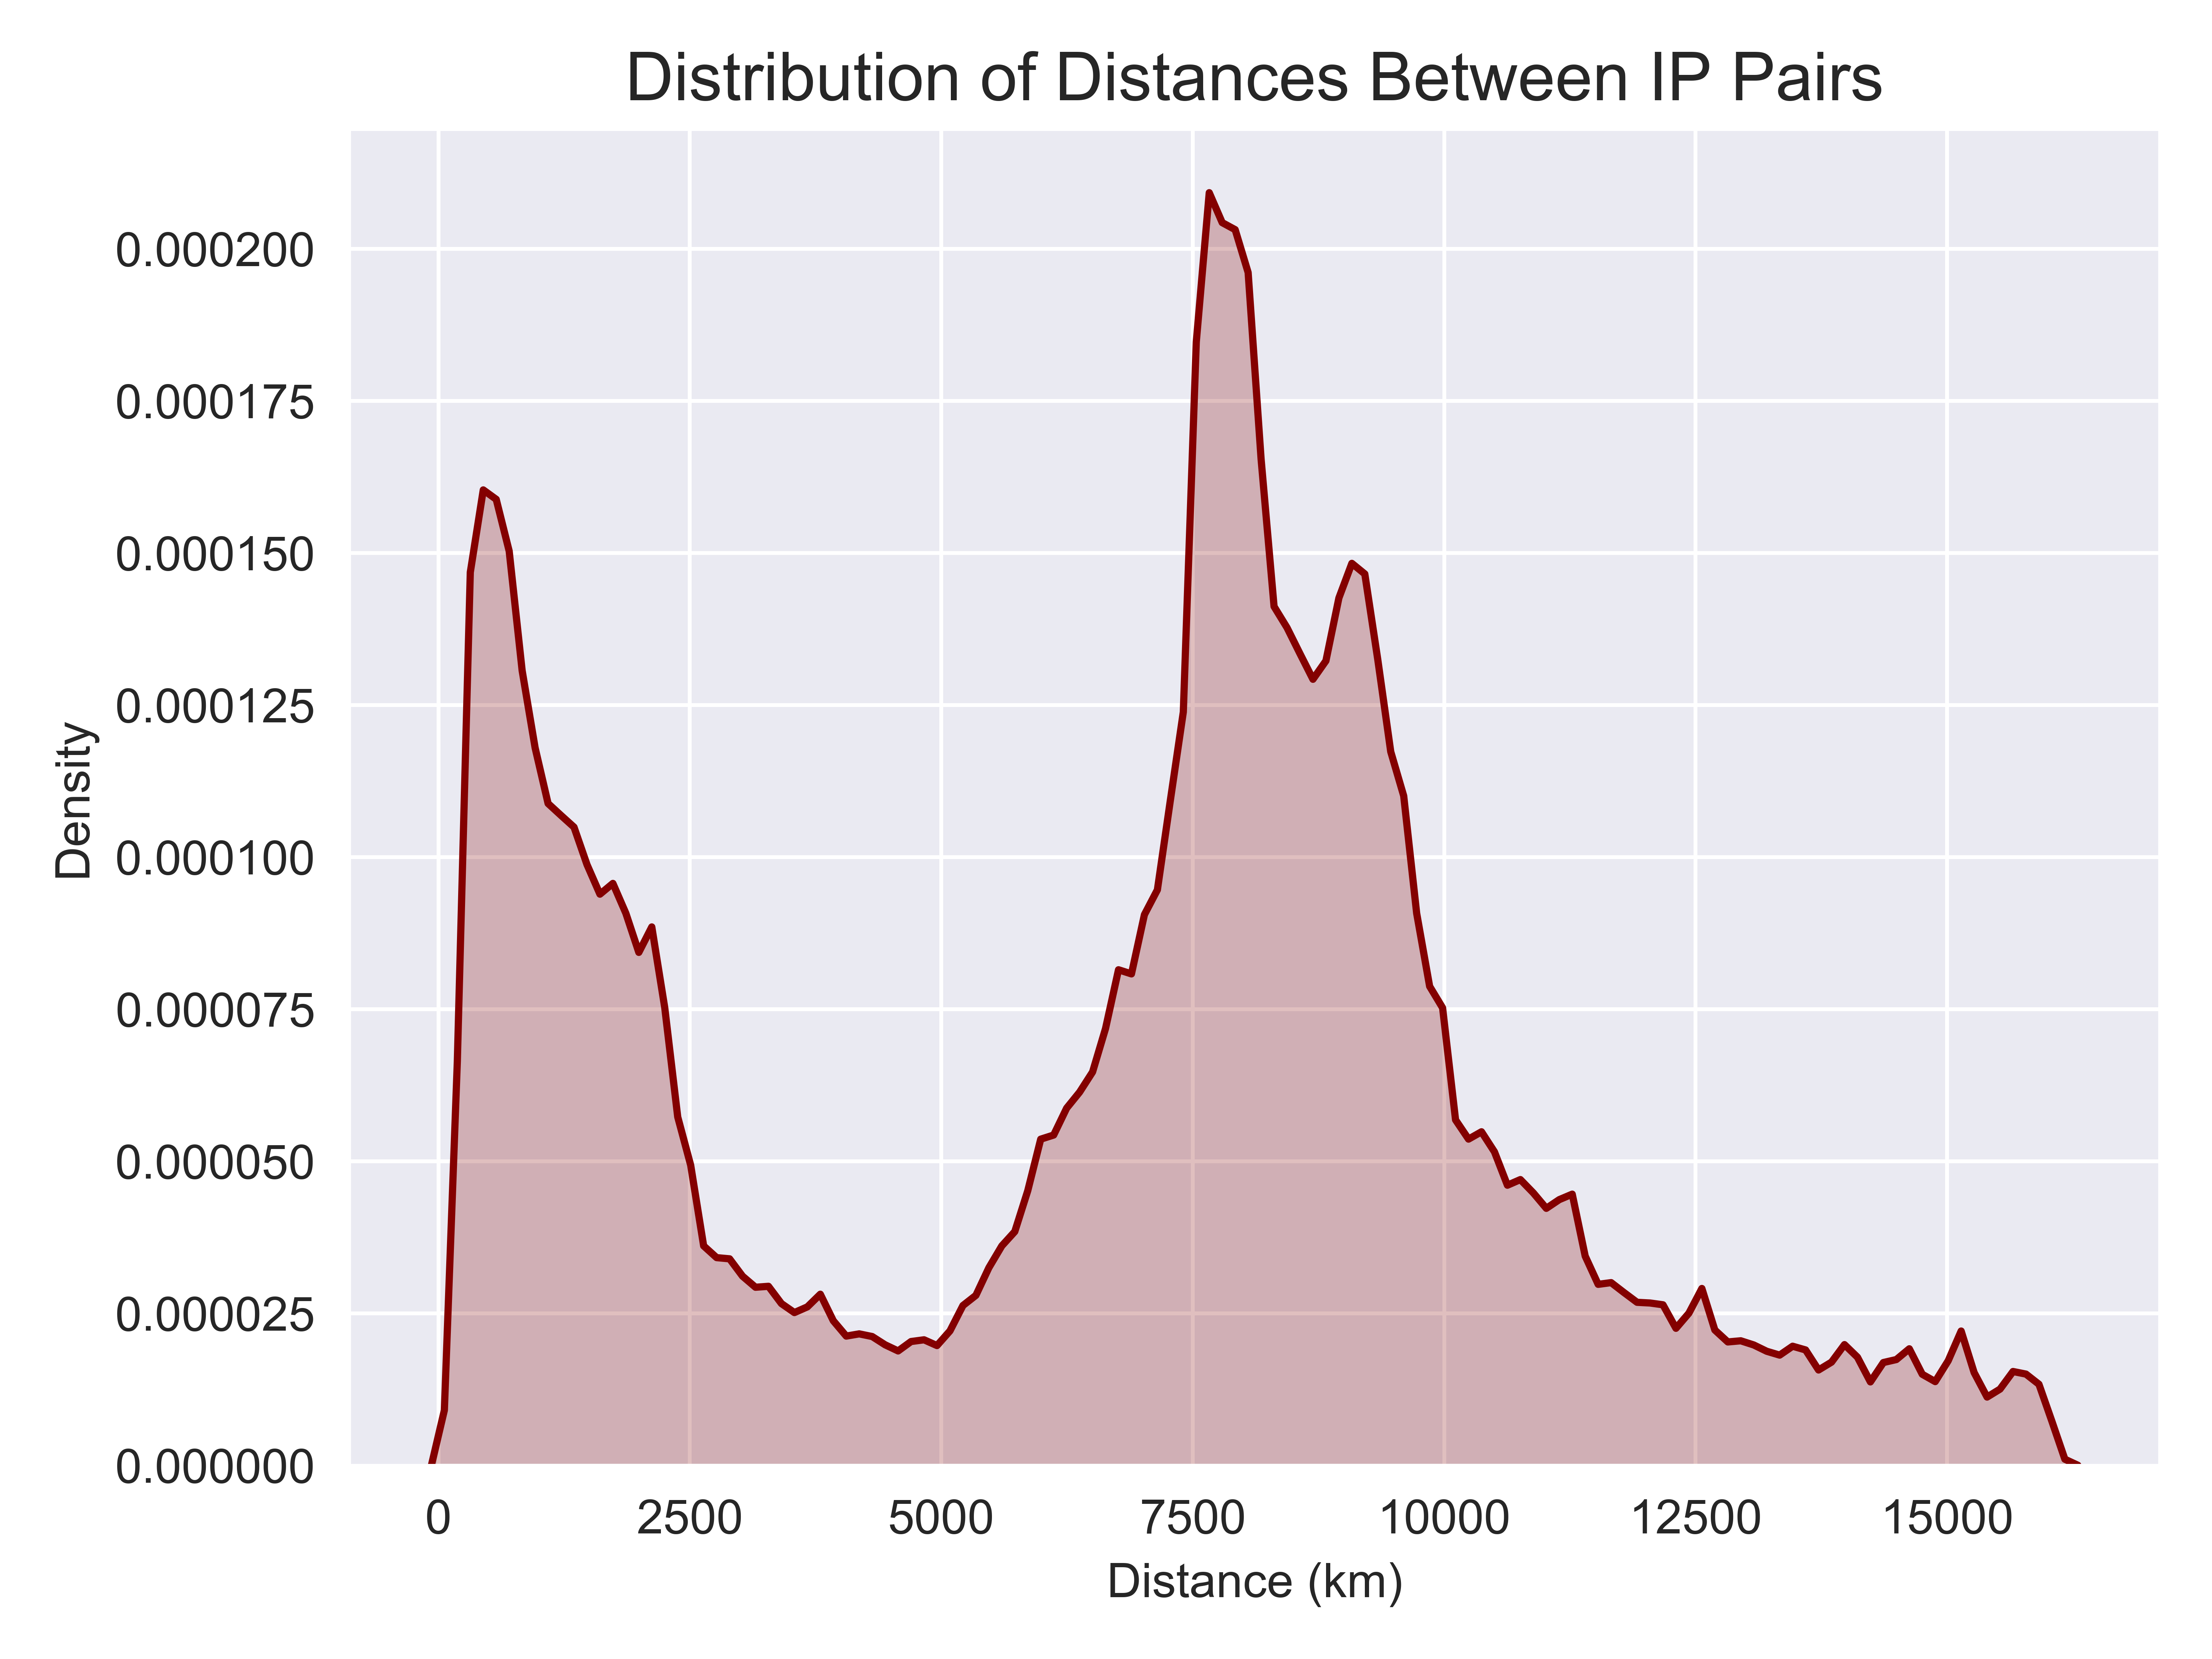
\includegraphics[width=0.75\textwidth]{caida/distance_distribution.png}
    \caption{Distribution of distance between IP pairs}
    \label{fig:caida_distance_distribution}
\end{figure}

Unfortunately the data from indirect ping calculation (see \autoref{sec:design_caida}) had to be discarded as they were deemed too unreliable. \autoref{fig:caida_rtt_distribution_indirect} shows the distribution of \rtts calculated using the indirect ping calculation method, of which a calculated \textapprox29\% are below zero. Since a significant fraction of the data points are completely impossible it was decided that this data was too reliable for further analysis. The remainder of the data analyses in this section are based on the direct ping calculation method only.

\begin{figure}[H]
    \centering
    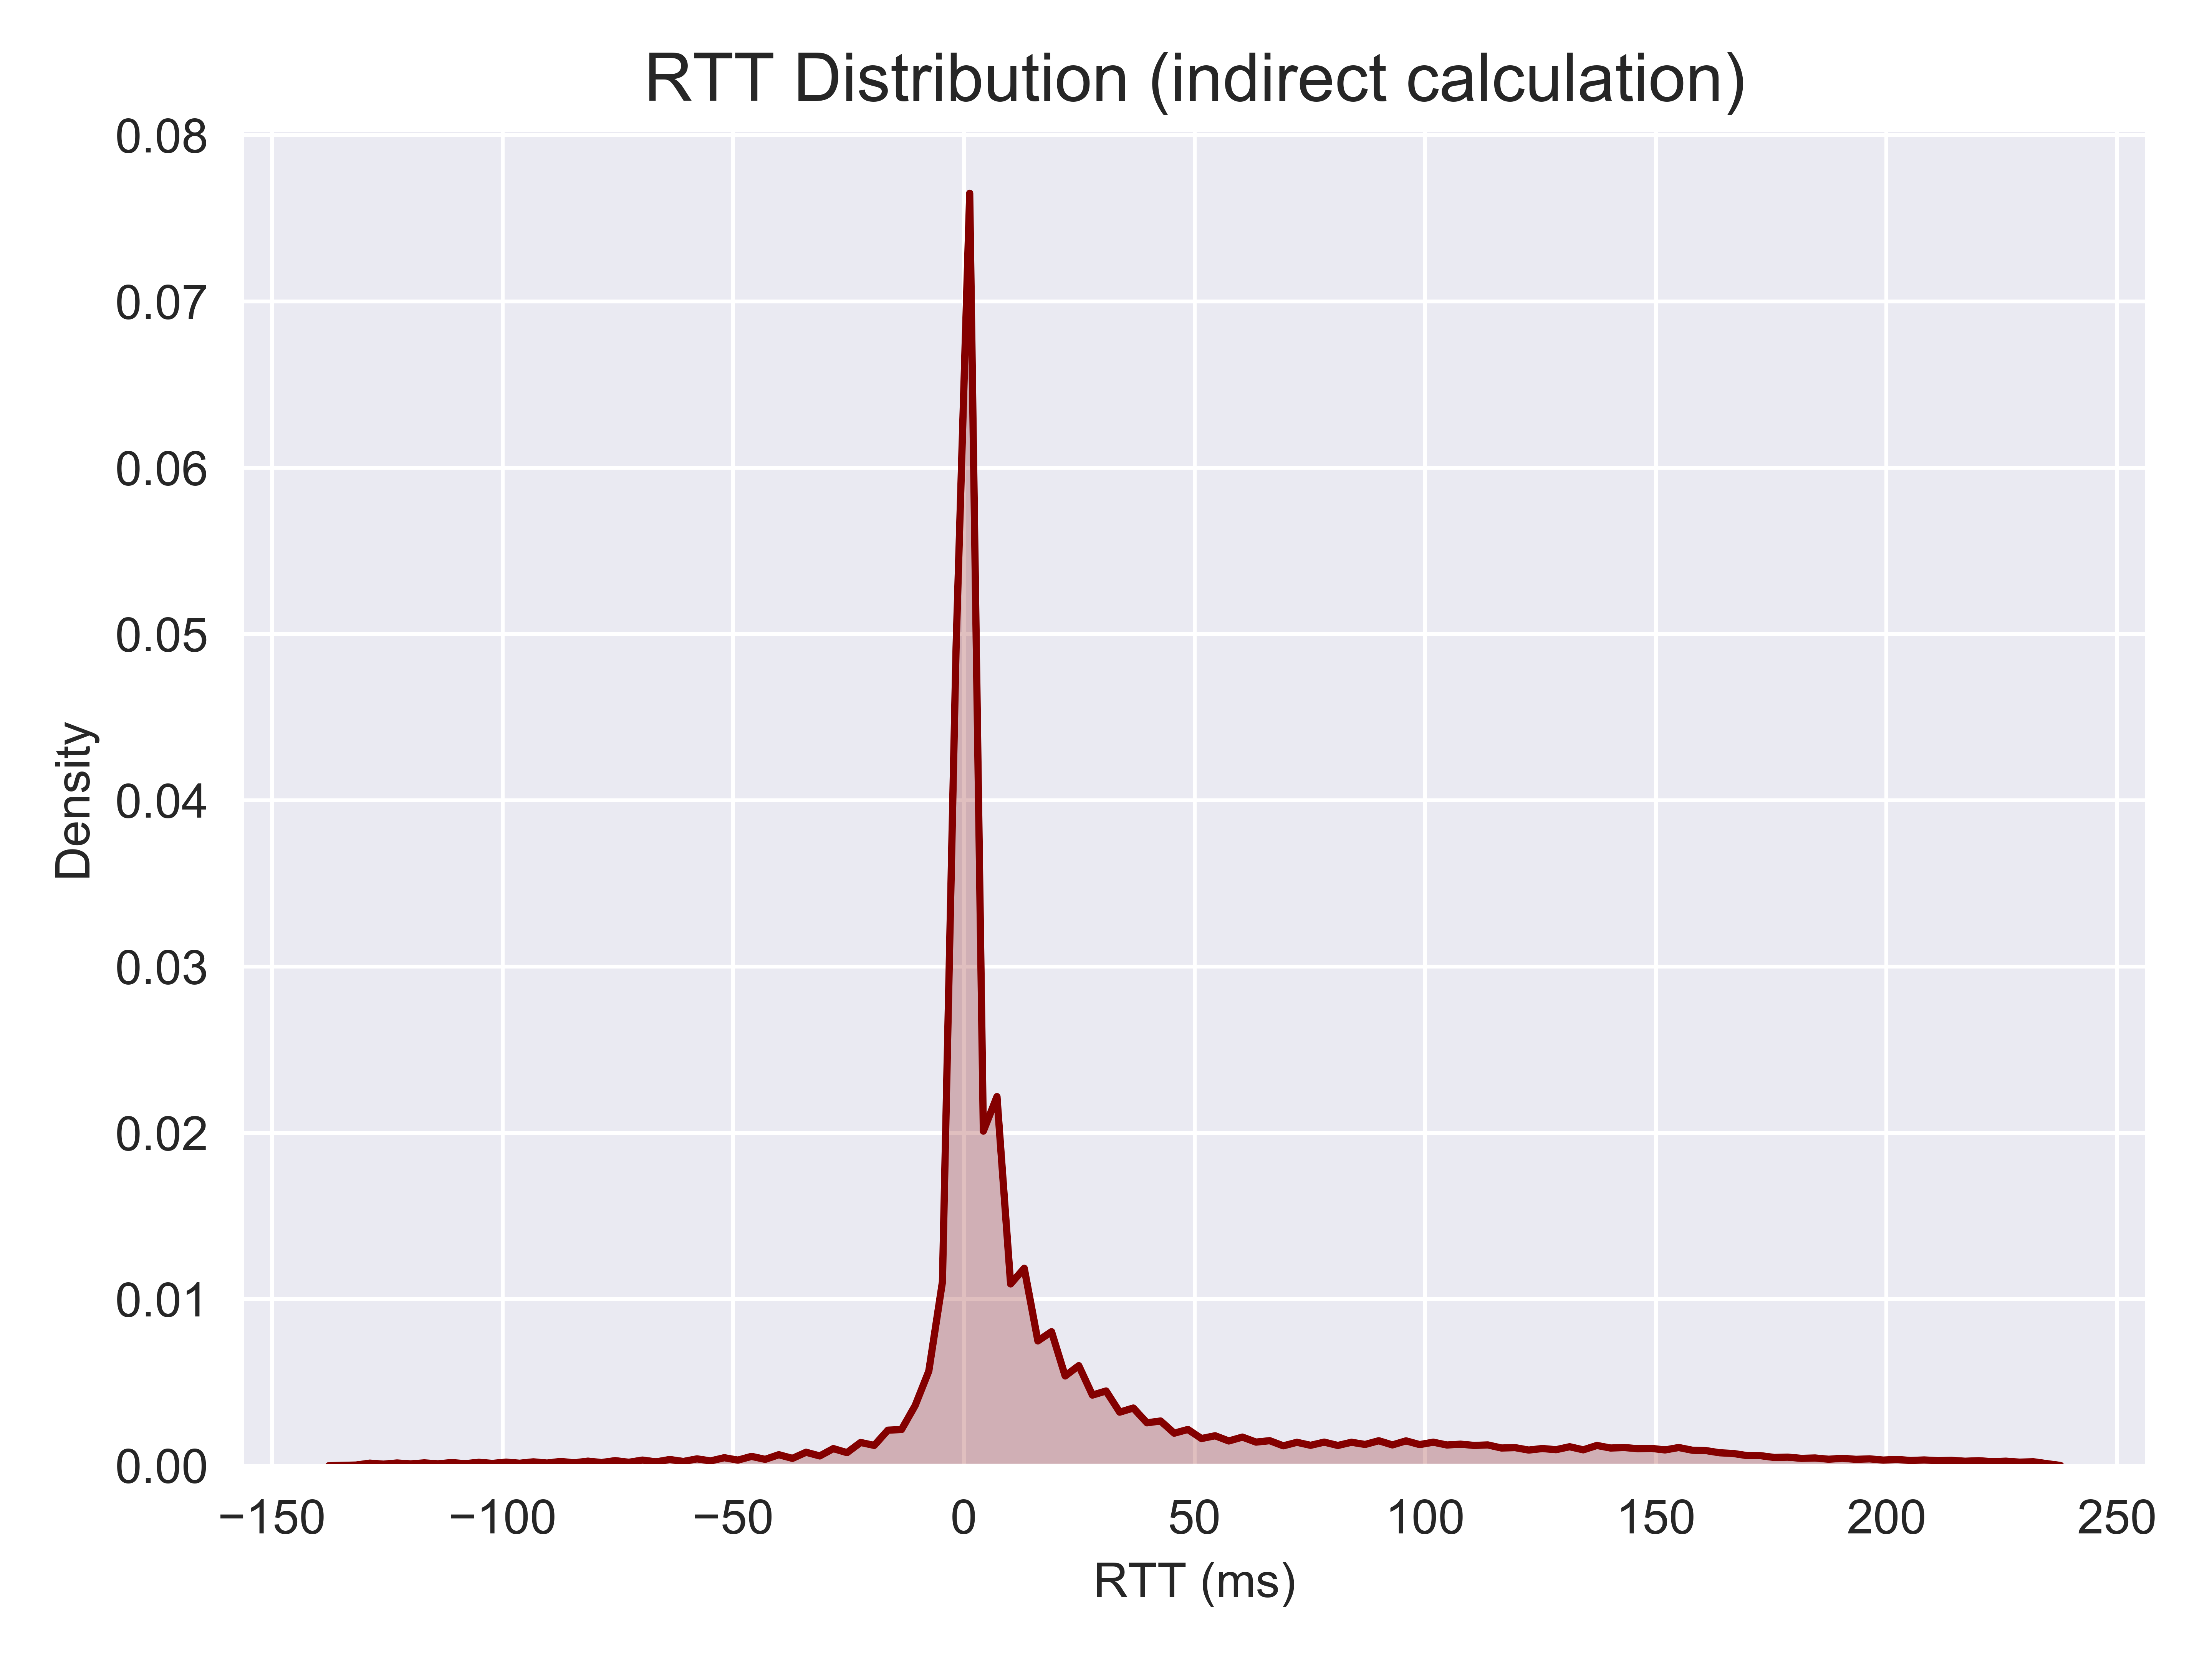
\includegraphics[width=0.75\textwidth]{caida/rtt_distribution_indirect.png}
    \caption{Distribution of RTT between IP pairs, indirect ping calculation}
    \label{fig:caida_rtt_distribution_indirect}
\end{figure}

To further assess data quality we turned to measures of the reliability of each data point. \autoref{fig:caida_measurements_distribution} shows the distribution of measurements count between each \ip pair, showing that although most \ip pairs had on the order of 1-20 measurements, a sizeable fraction had more than that, and there were even some in the 500+ measurements range. This is hypothesized to be the result of the way \ripe Atlas and \caida nodes are networked. A node's local gateway would always show up on a \gls{traceroute} (unless configured to not respond to pings) as would common paths through a node's \isp, so these \ips are likely measured extremely frequently.

\begin{figure}[H]
    \centering
    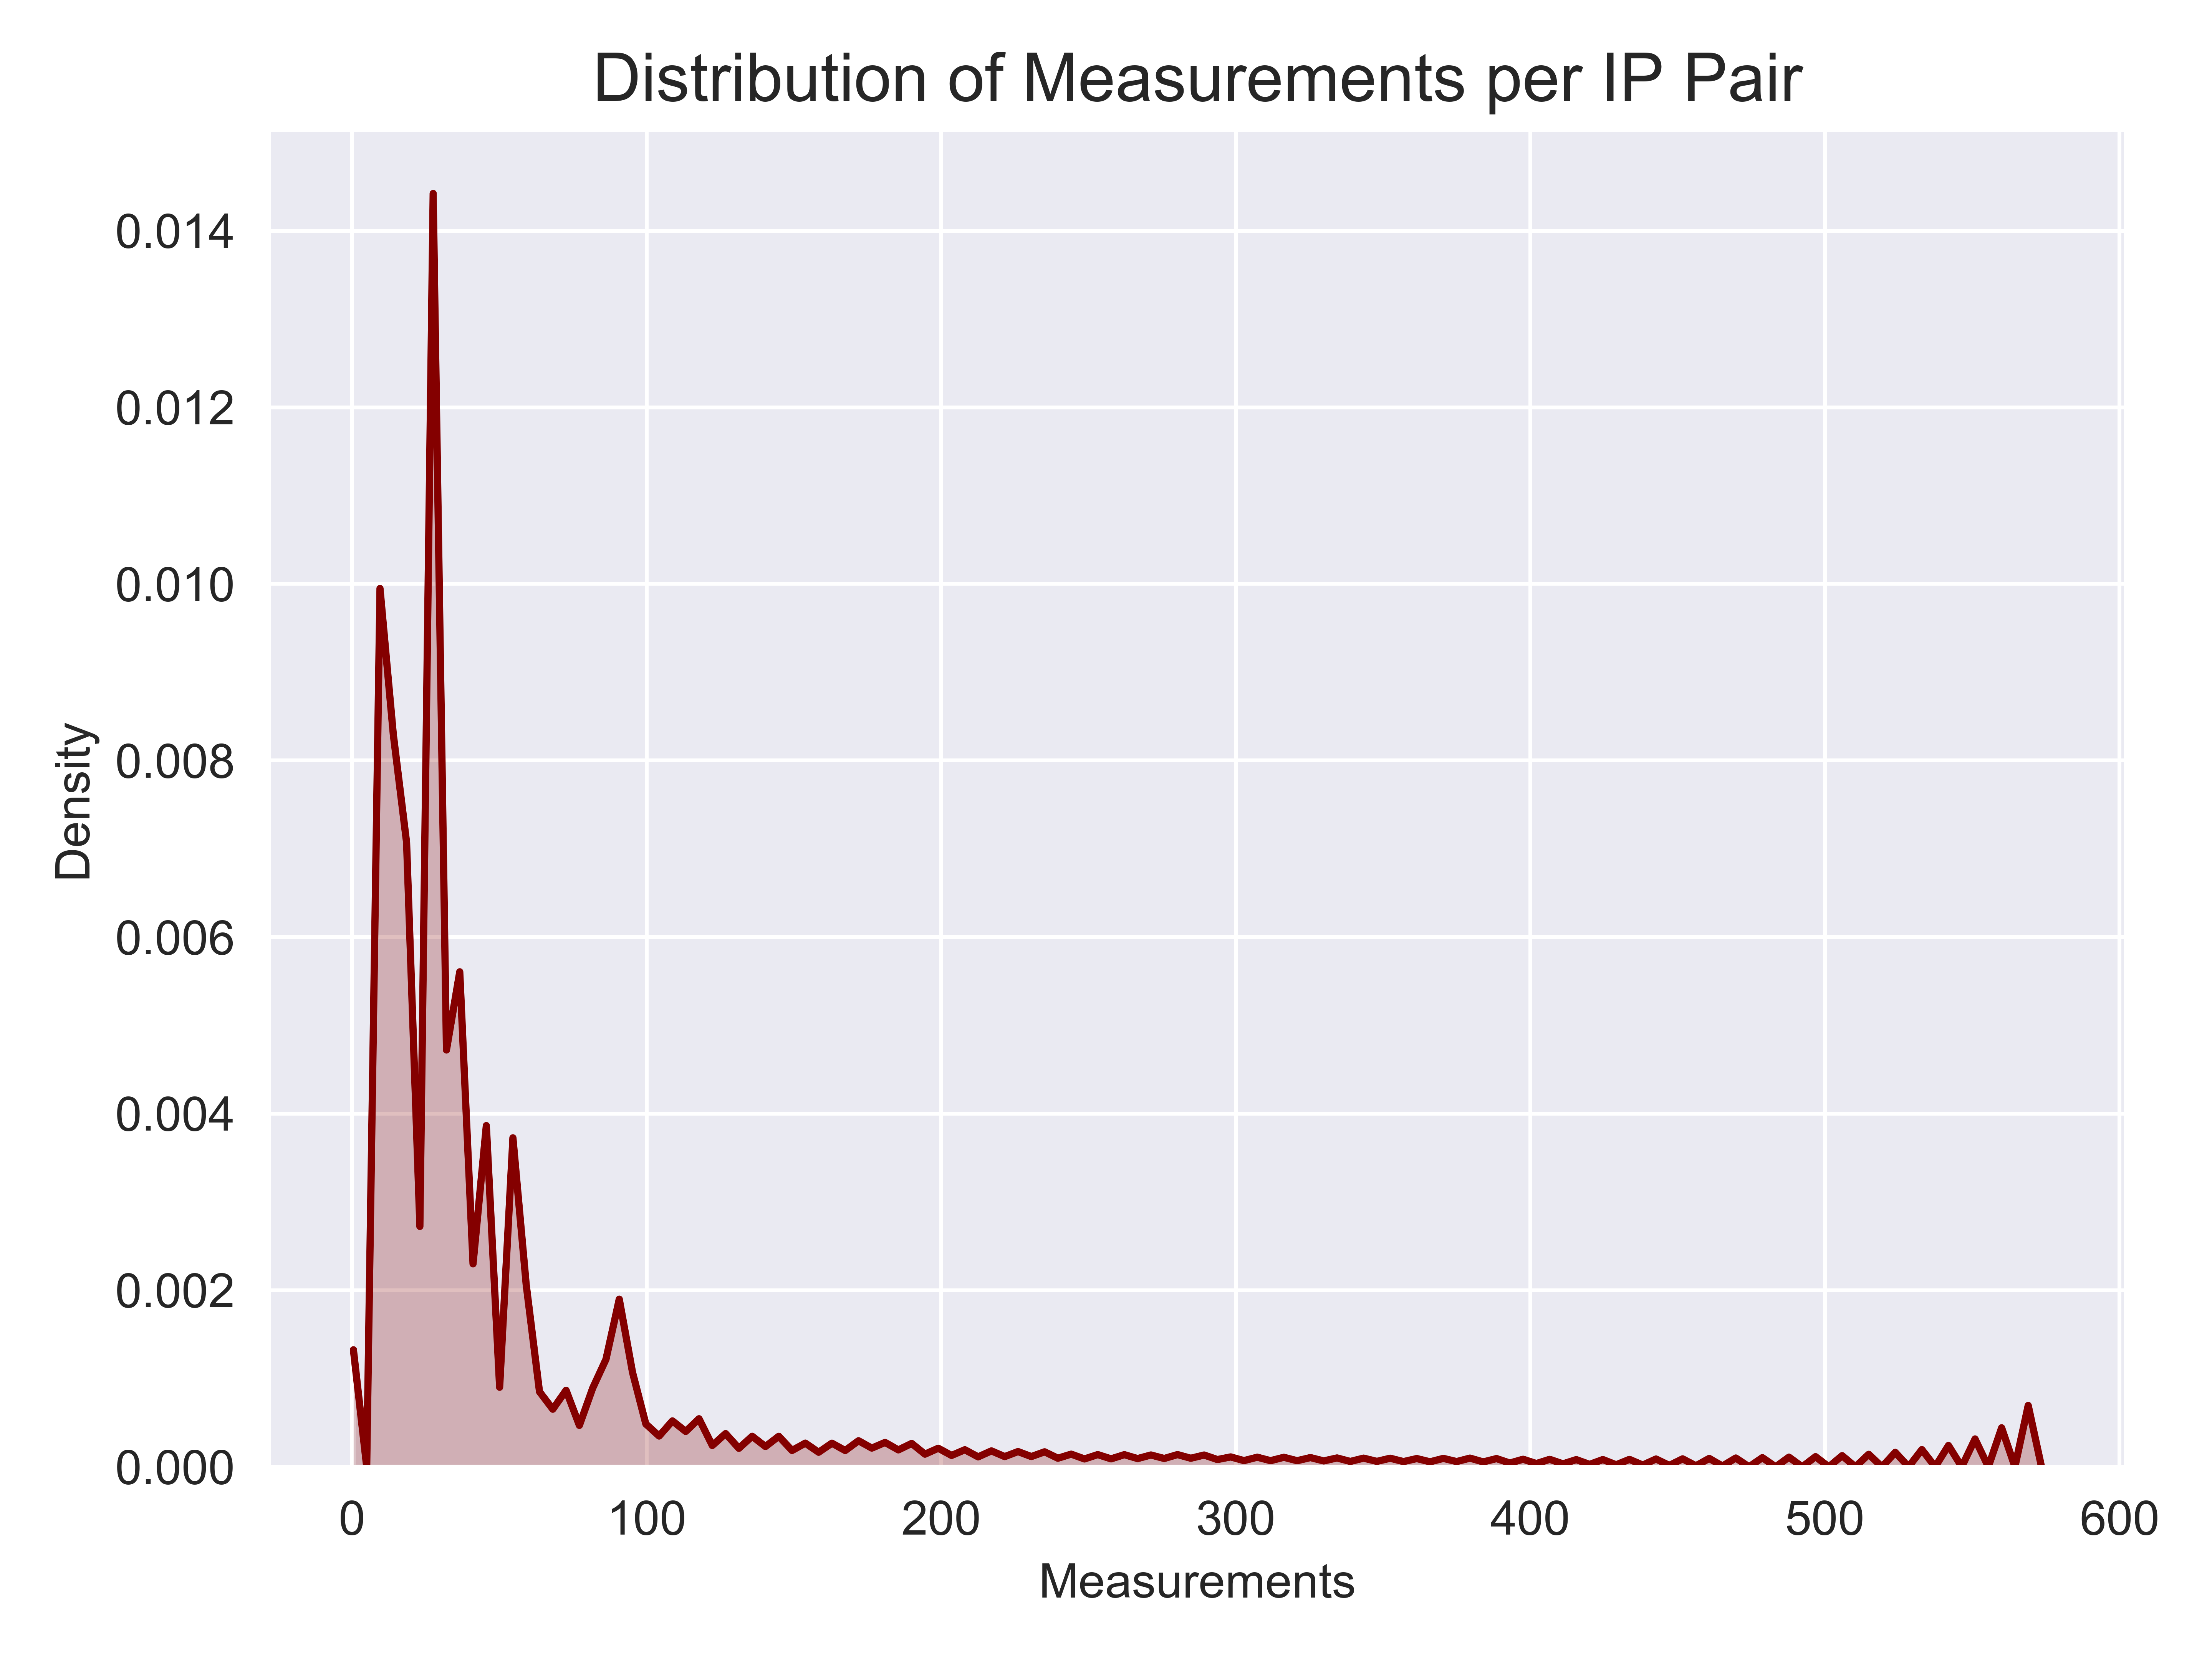
\includegraphics[width=0.75\textwidth]{caida/measurements_distribution.png}
    \caption{Distribution of measurements count for each IP pair}
    \label{fig:caida_measurements_distribution}
\end{figure}

\begin{figure}[H]
    \centering
    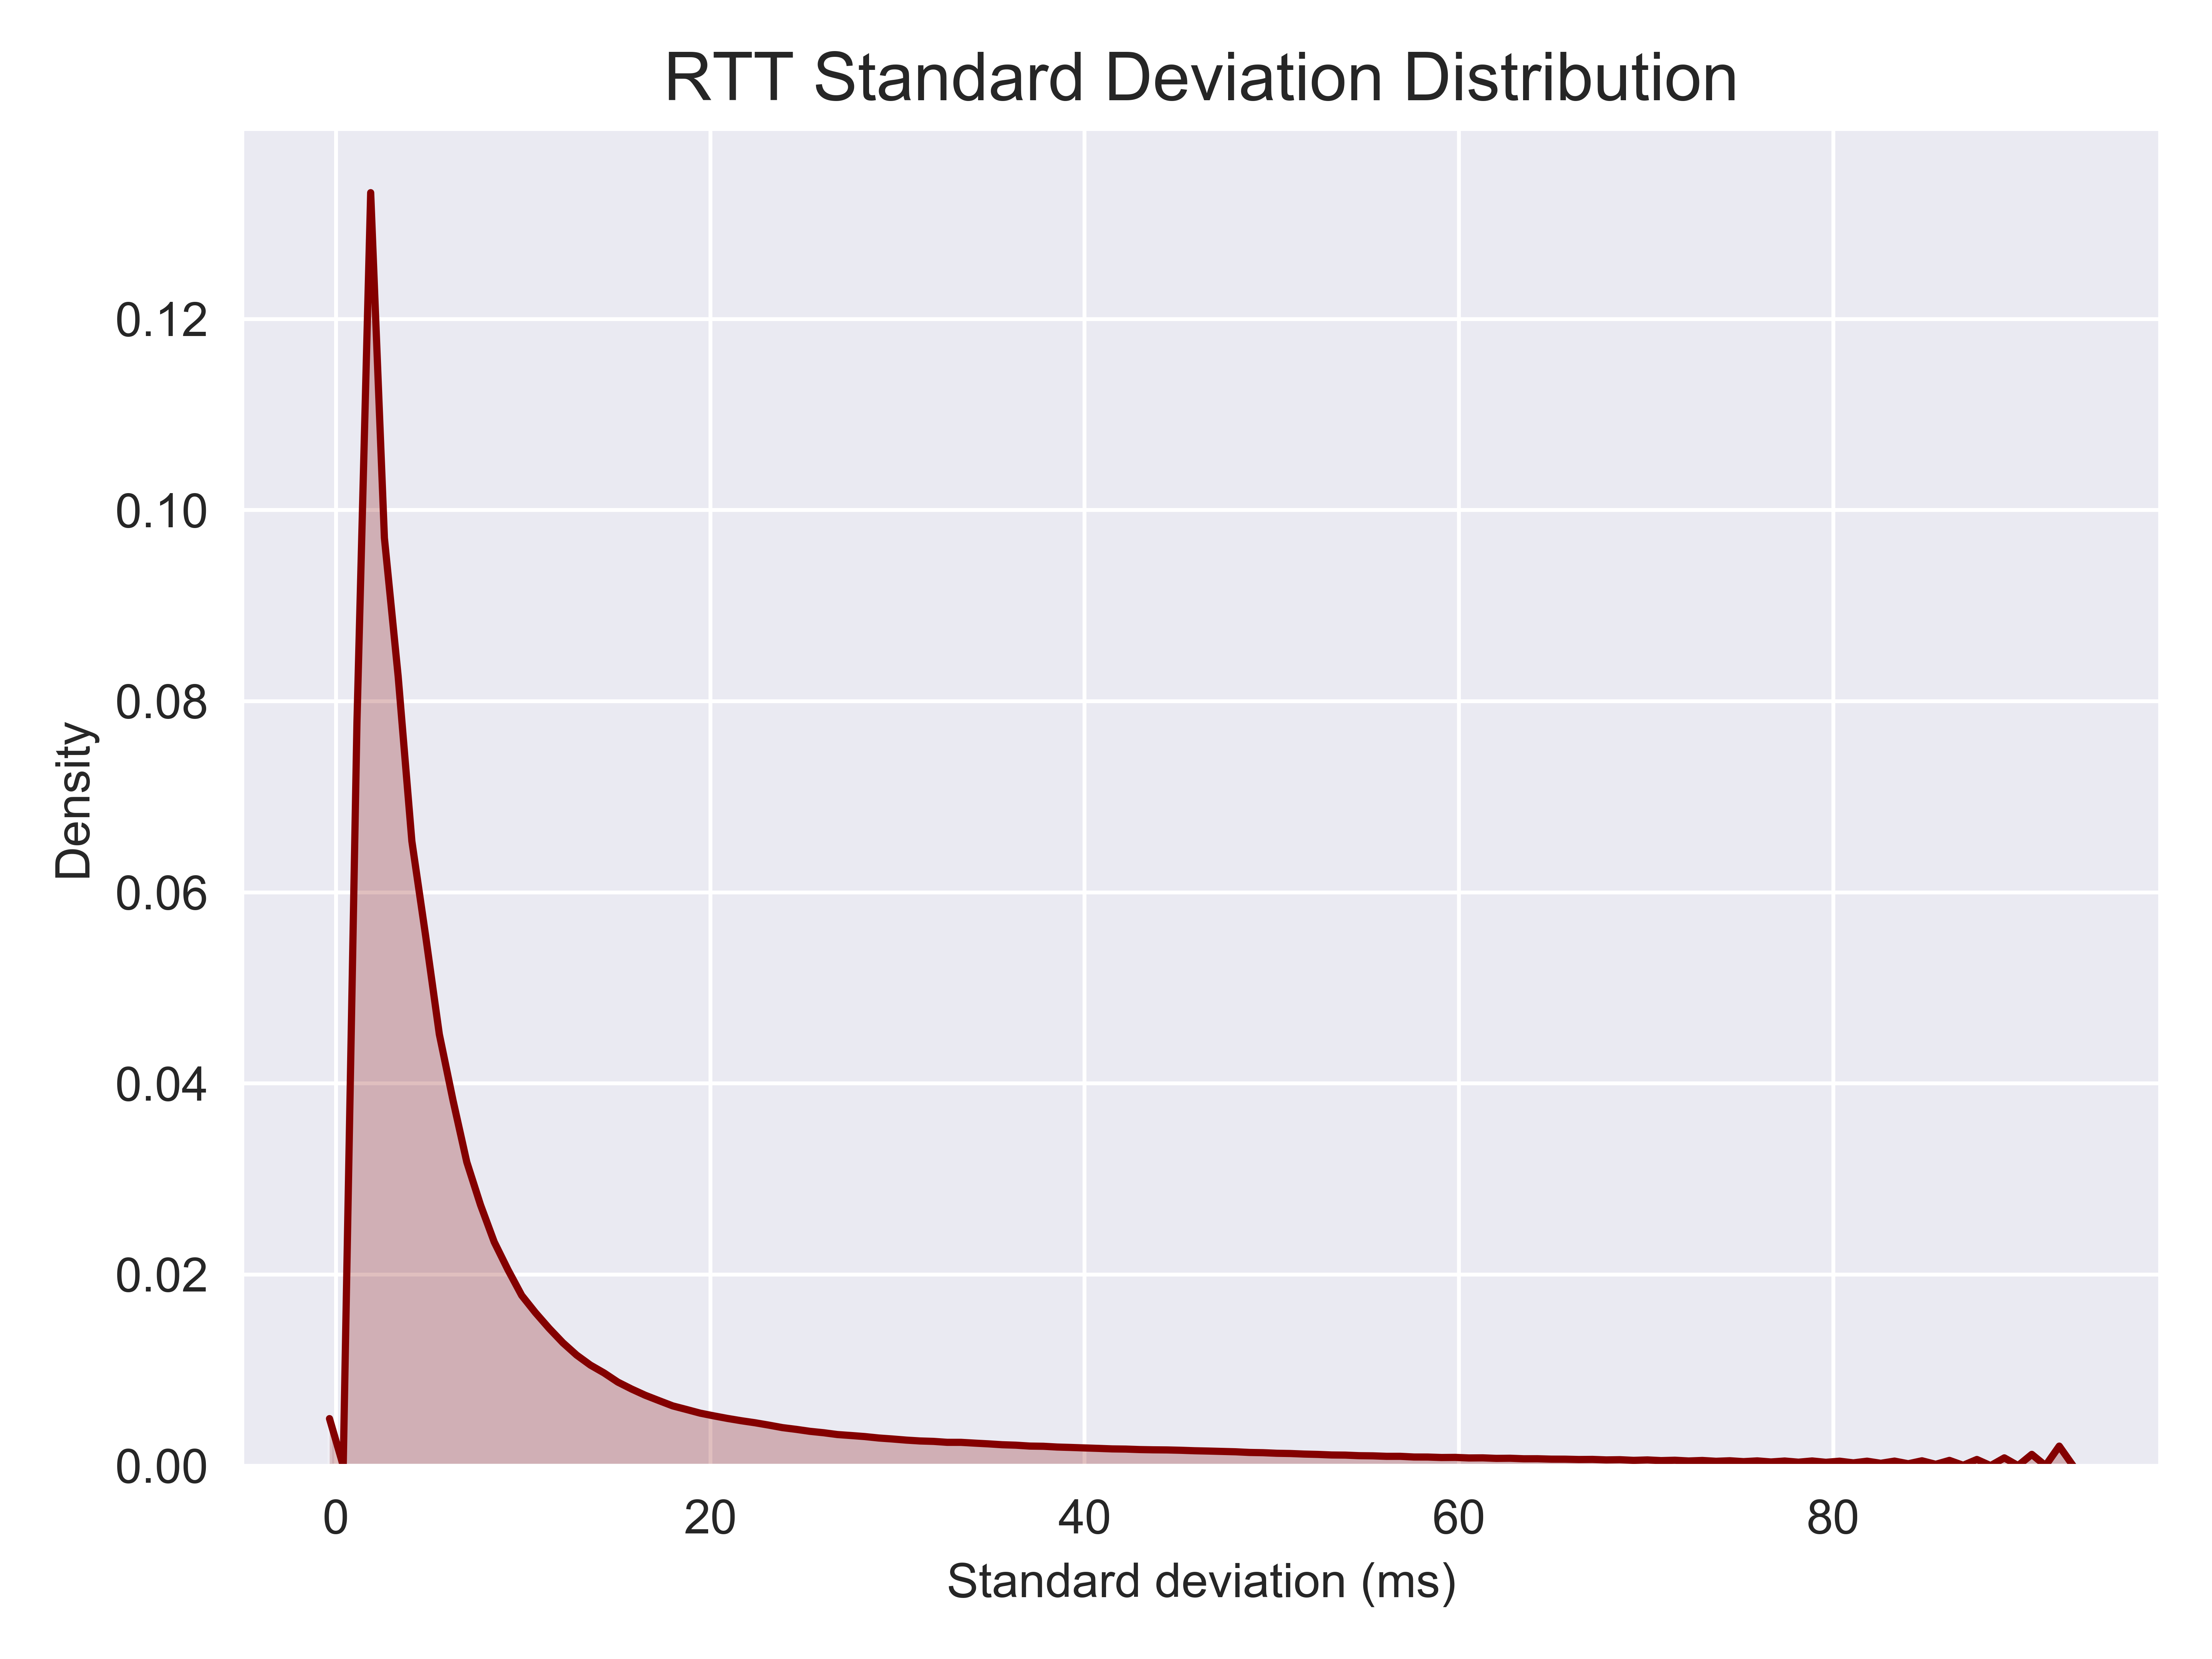
\includegraphics[width=0.75\textwidth]{caida/rtt_stdev_distribution.png}
    \caption{Distribution of IP pair standard deviations}
    \label{fig:caida_stdev_distribution}
\end{figure}

To assess the quality of the measurements for each \ip pair we first turn to the standard deviation. \autoref{fig:caida_stdev_distribution} shows the distribution of standard deviations across all measured \ip pairs (for charting purposes, pairs with only one measurement were interpreted as 0 standard deviation). The chart shows an incredibly smooth curve in with the overwhelming majority of pairs having standard deviations well below 20 ms. To further improve upon that analysis we next turned to \cvs as a measurement of data quality. \cvs are a dimensionless measure that can be interpreted the same across any data set, where lower means better. \autoref{fig:caida_cv_distribution} shows the distribution of \cvs for all \ip pairs, with the majority of \cvs below 0.1 --- in other words, very good data with low spread.

\begin{figure}[H]
    \centering
    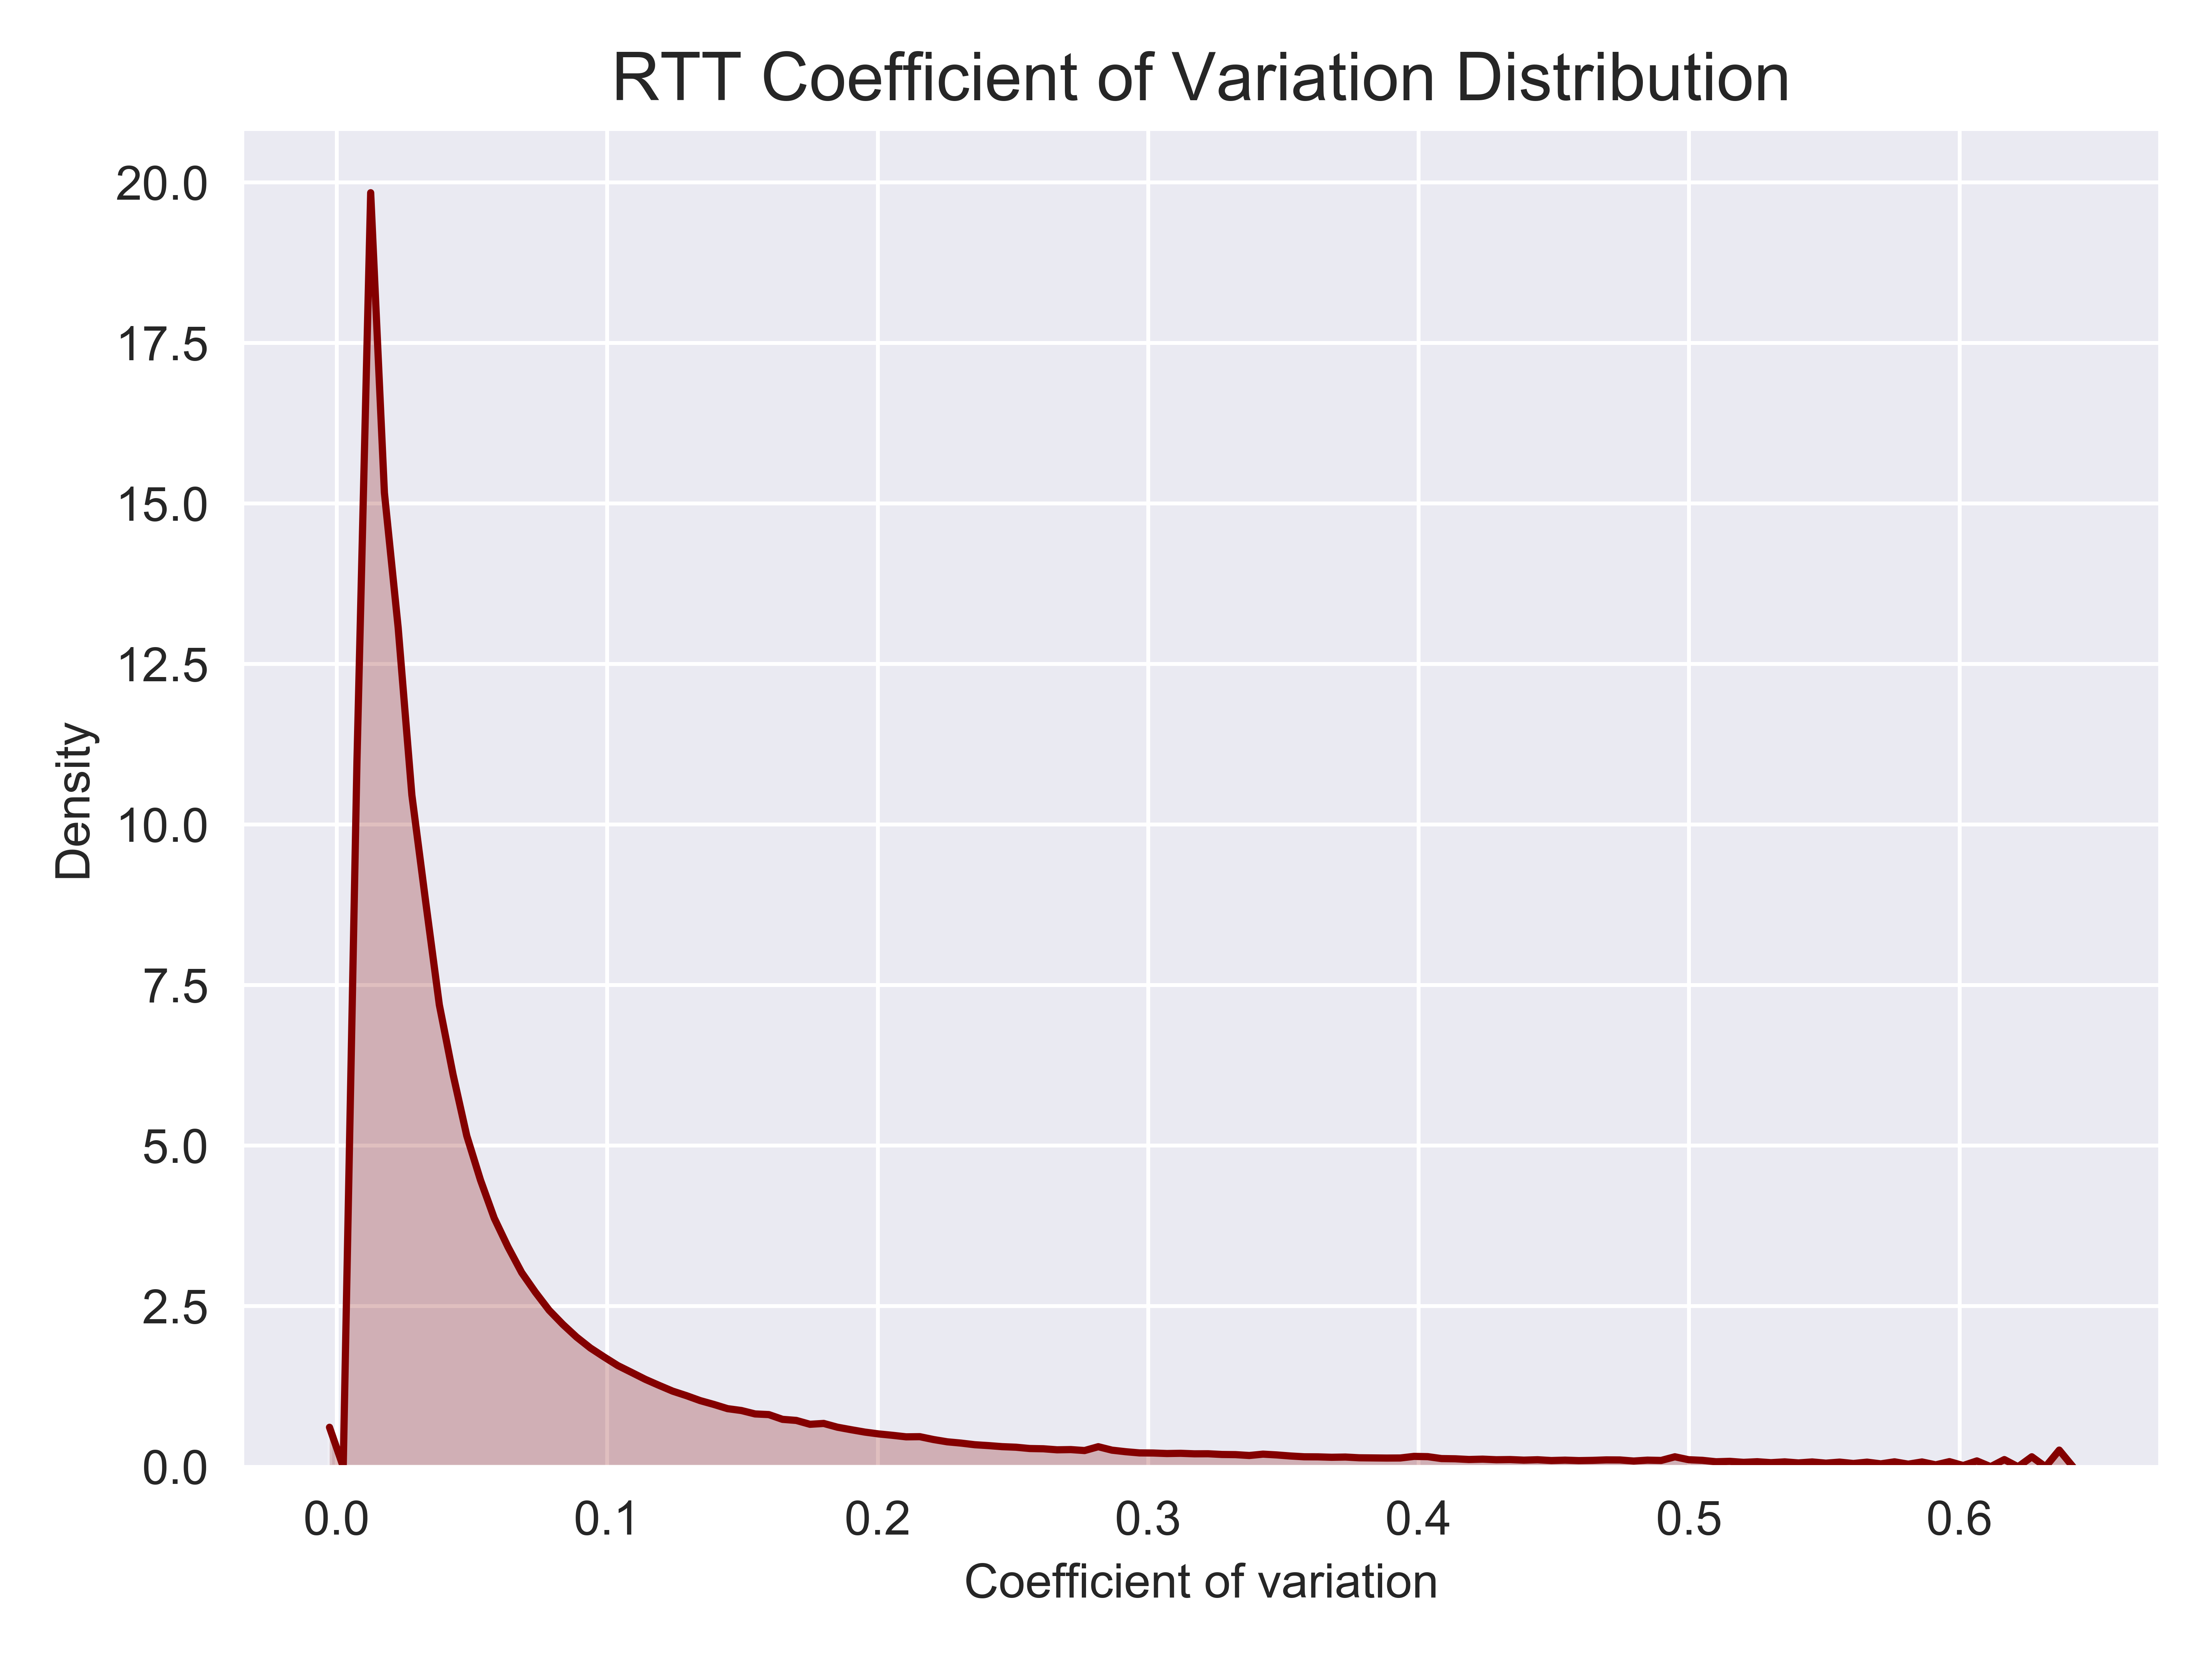
\includegraphics[width=0.75\textwidth]{caida/rtt_cv_distribution.png}
    \caption{Distribution of IP pair coefficients of variation}
    \label{fig:caida_cv_distribution}
\end{figure}

\subsection{Primitive Connectivity Analyses}

Each data point comprises an \ip pair, but each destination \ip --- that is, each \ip that a \caida or \ripe atlas node ran a measurement against --- appears many times, at least once for every node that ran a measurement against it. Averaging these won't work (it makes little sense to average together measurements from a server in Boston with a server in Moscow against a server in New York, since the Moscow measurement node will naturally report a much higher \rtt), so normalization is needed. The first normalization attempted was simple normalization by distance, which returns values in \si{\milli\second\per\kilo\meter} since milliseconds and kilometers are natural units for \rtts and distance, respectively.

\begin{figure}
    \centering
    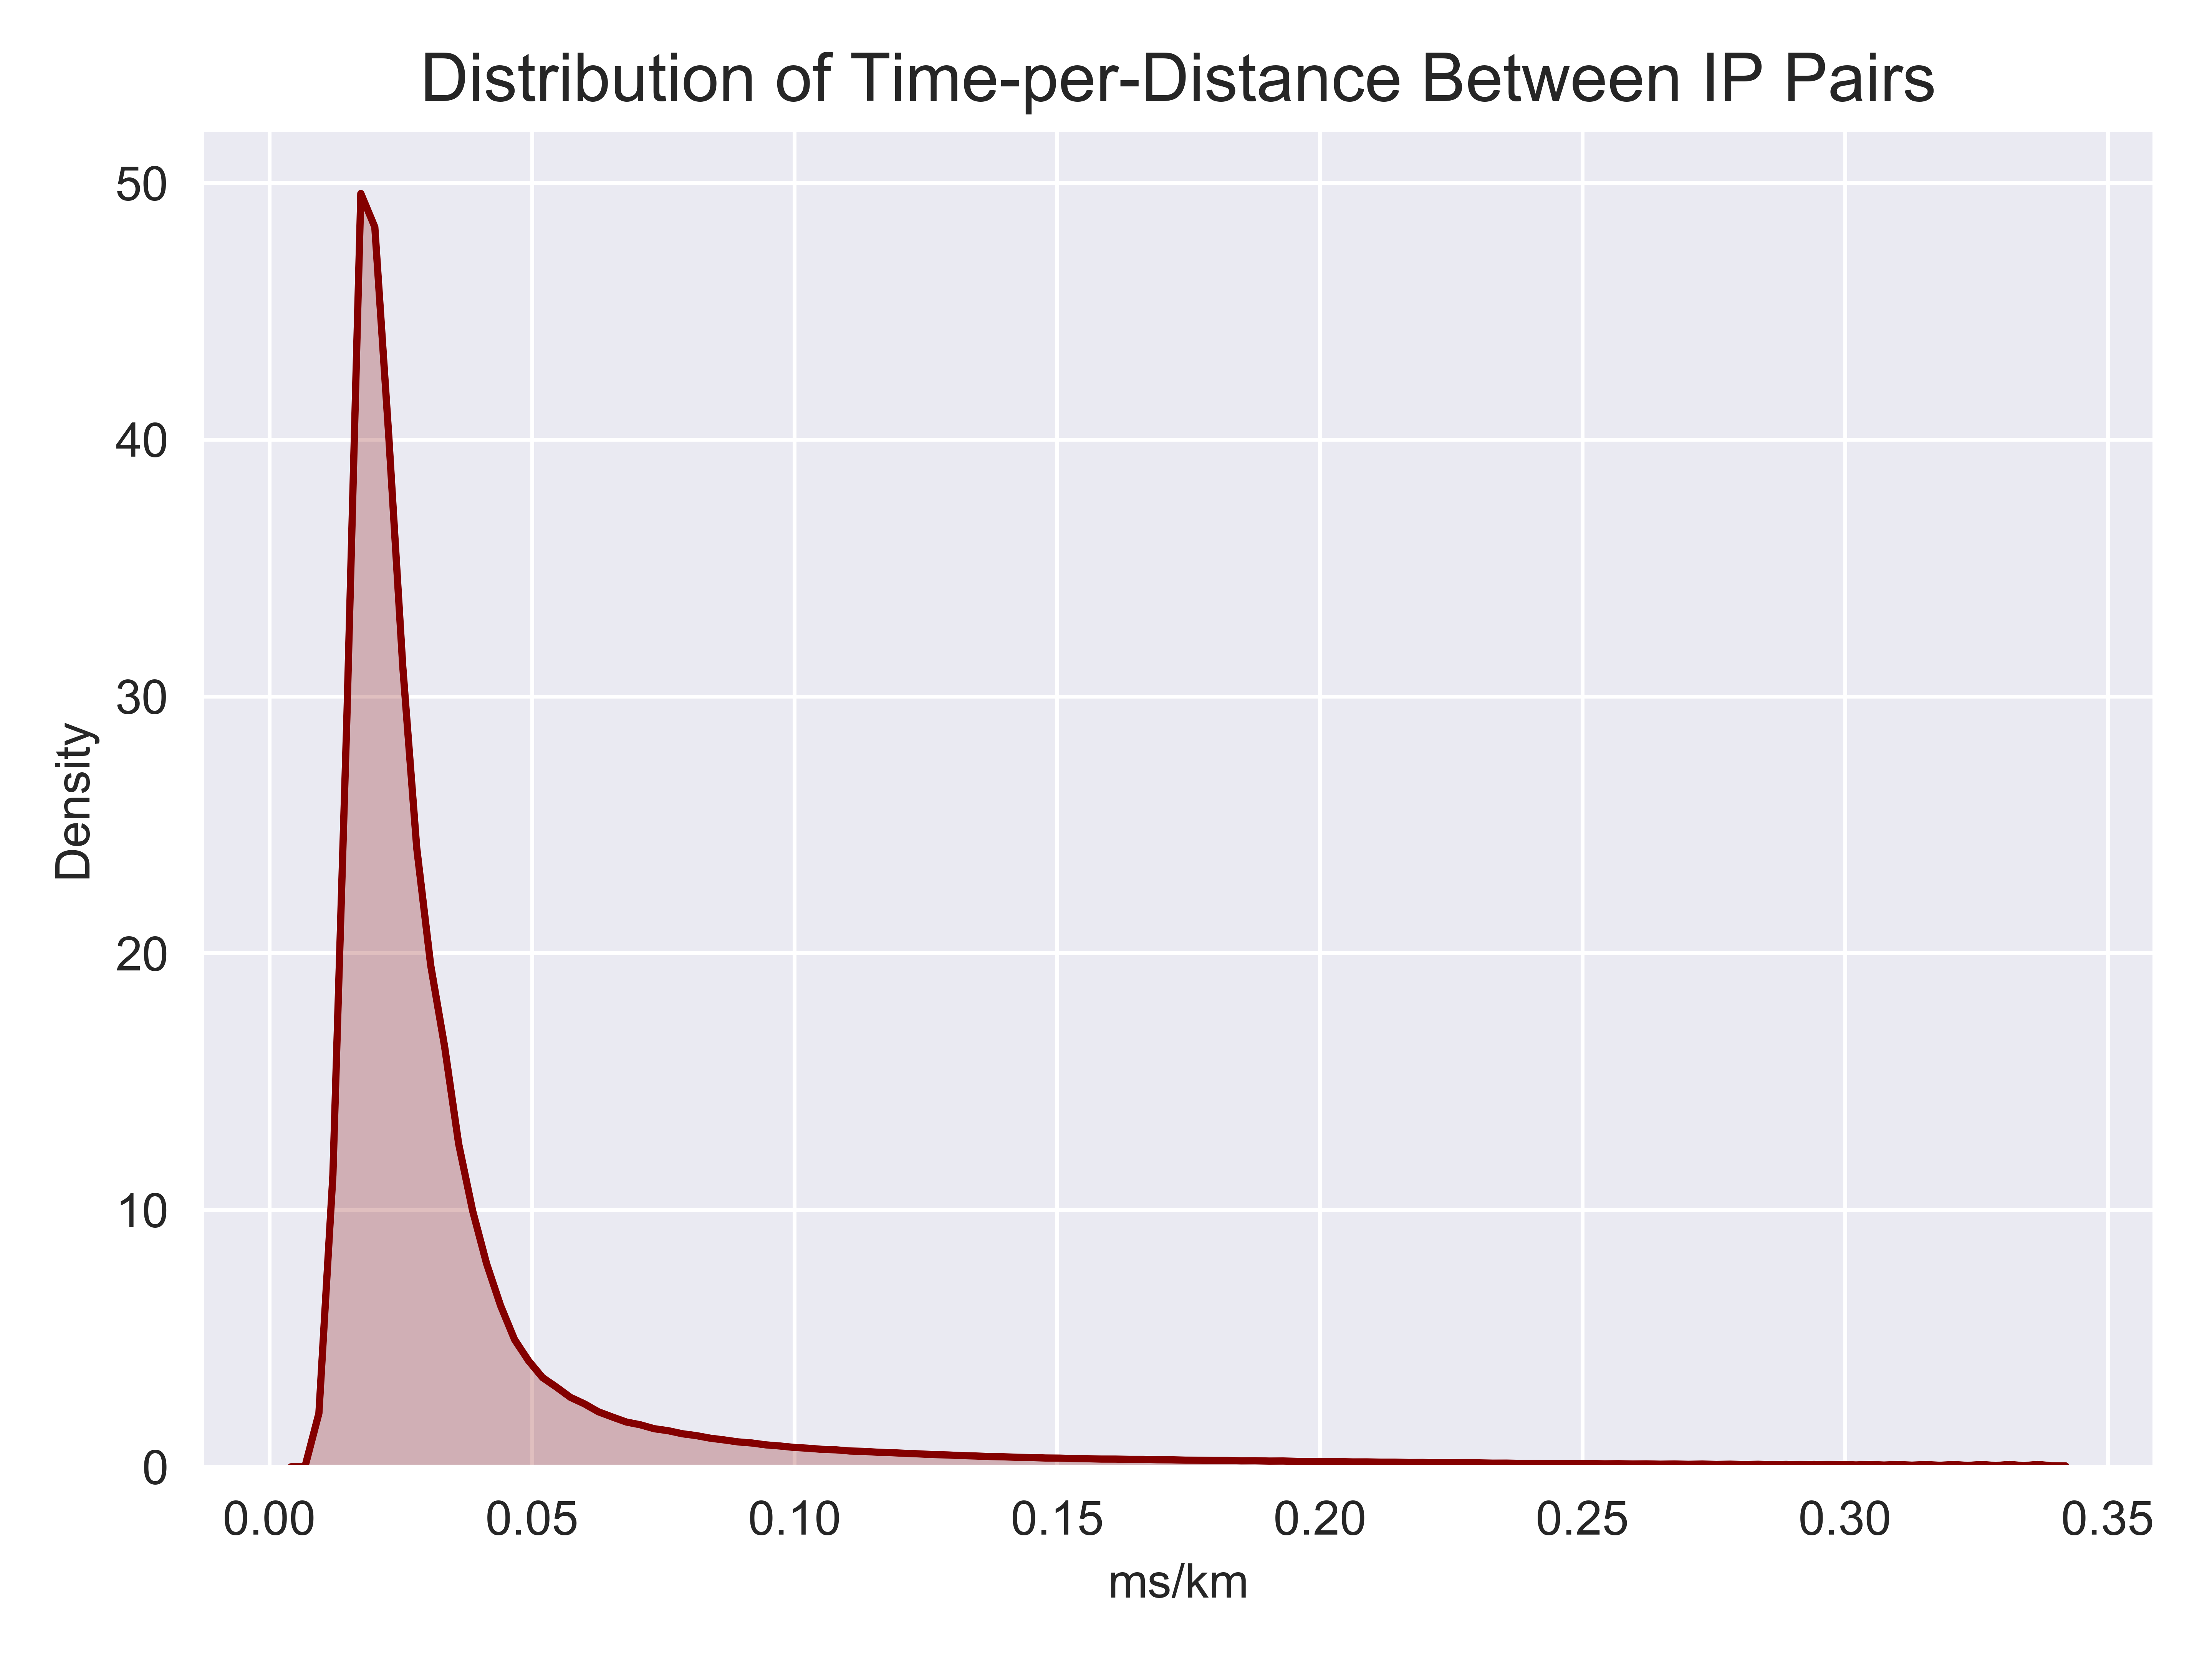
\includegraphics[width=0.75\textwidth]{caida/ms_per_km_distribution.png}
    \caption{Distribution of milliseconds-per-kilometer connectivities}
    \label{fig:caida_ms_per_km_distribution}
\end{figure}

The \si{\milli\second\per\kilo\meter} distribution shown in \autoref{fig:caida_ms_per_km_distribution} is remarkably uninformative on its own, but it does demonstrate an important feature. Normalization succeeds in removing the bimodality of the \rtt distribution shown in \autoref{fig:caida_rtt_distribution} without removing \textit{all} the spread of the data. This both further affirms the earlier hypothesis about the cause of the bimodality and gives cause to believe that geographic charting may yield interesting results.

Unfortunately this metric is challenging to chart with any color scale. The majority of values are between 0.0 and 0.05 \si{\milli\second\per\kilo\meter} but values an order of magnitiude higher must also be charted, and a log scale fails to capture important data. To solve this, a new metric based on efficiency relative to the speed of light was devised.

The speed of light is \SI{299.79246}{\kilo\meter\per\milli\second} (shown in milliseconds and kilometers for ease of distance and relevance to \rtts), so the theoretical minimum \rtt between two points \textapprox 300 km apart is \textapprox2 milliseconds -- one millisecond one way, another on the return trip. All telecommunications happens over electromagnetic mediums, be it fibre optic cables or copper wires, and thus have a transmission delay equal to the speed of light. If the \rtt was higher than 2 milliseconds, there must logically be some loss somewhere in the network, whether that means poor infrastructure or wiring that doesn't follow a straight line to the source -- either way, an inefficiency. The smaller the \rtt, the higher the efficiency, and vice versa. This has the desirable quality that extreme outliers are always between 0 and 1 regardless of how high the \rtt is. The formula for speed-of-light-efficiency based on \rtts is shown in formula \ref{form:speed_of_light_efficiency}.

\begin{formula}[H]
    \begin{equation}
        E = \frac{2d}{t \times 299.79246}
    \end{equation}
    \caption[Formula for speed-of-light efficiency]{Formula for speed-of-light efficiency; $E$ is efficiency as a scalar from 0-1, $d$ is distance in kilometers, and $t$ is the \rtt in milliseconds.}
    \label{form:speed_of_light_efficiency}
\end{formula}

Speed-of-light efficiency can also be thought of as a scalar multiplied by $c$, the speed of light -- it's the equivalent "speed" of a ping. With an improved normalization scheme to work with, subtle differences and patterns can be seen in the data,
as shown in \autoref{fig:speed_of_light_efficiency_distribution}. Also important is that this normalization technique provides with another means of filtering data -- anything above 1.0 efficiency can be removed since it violates the laws of physics by exceeding the speed of light.

\begin{figure}[H]
    \centering
    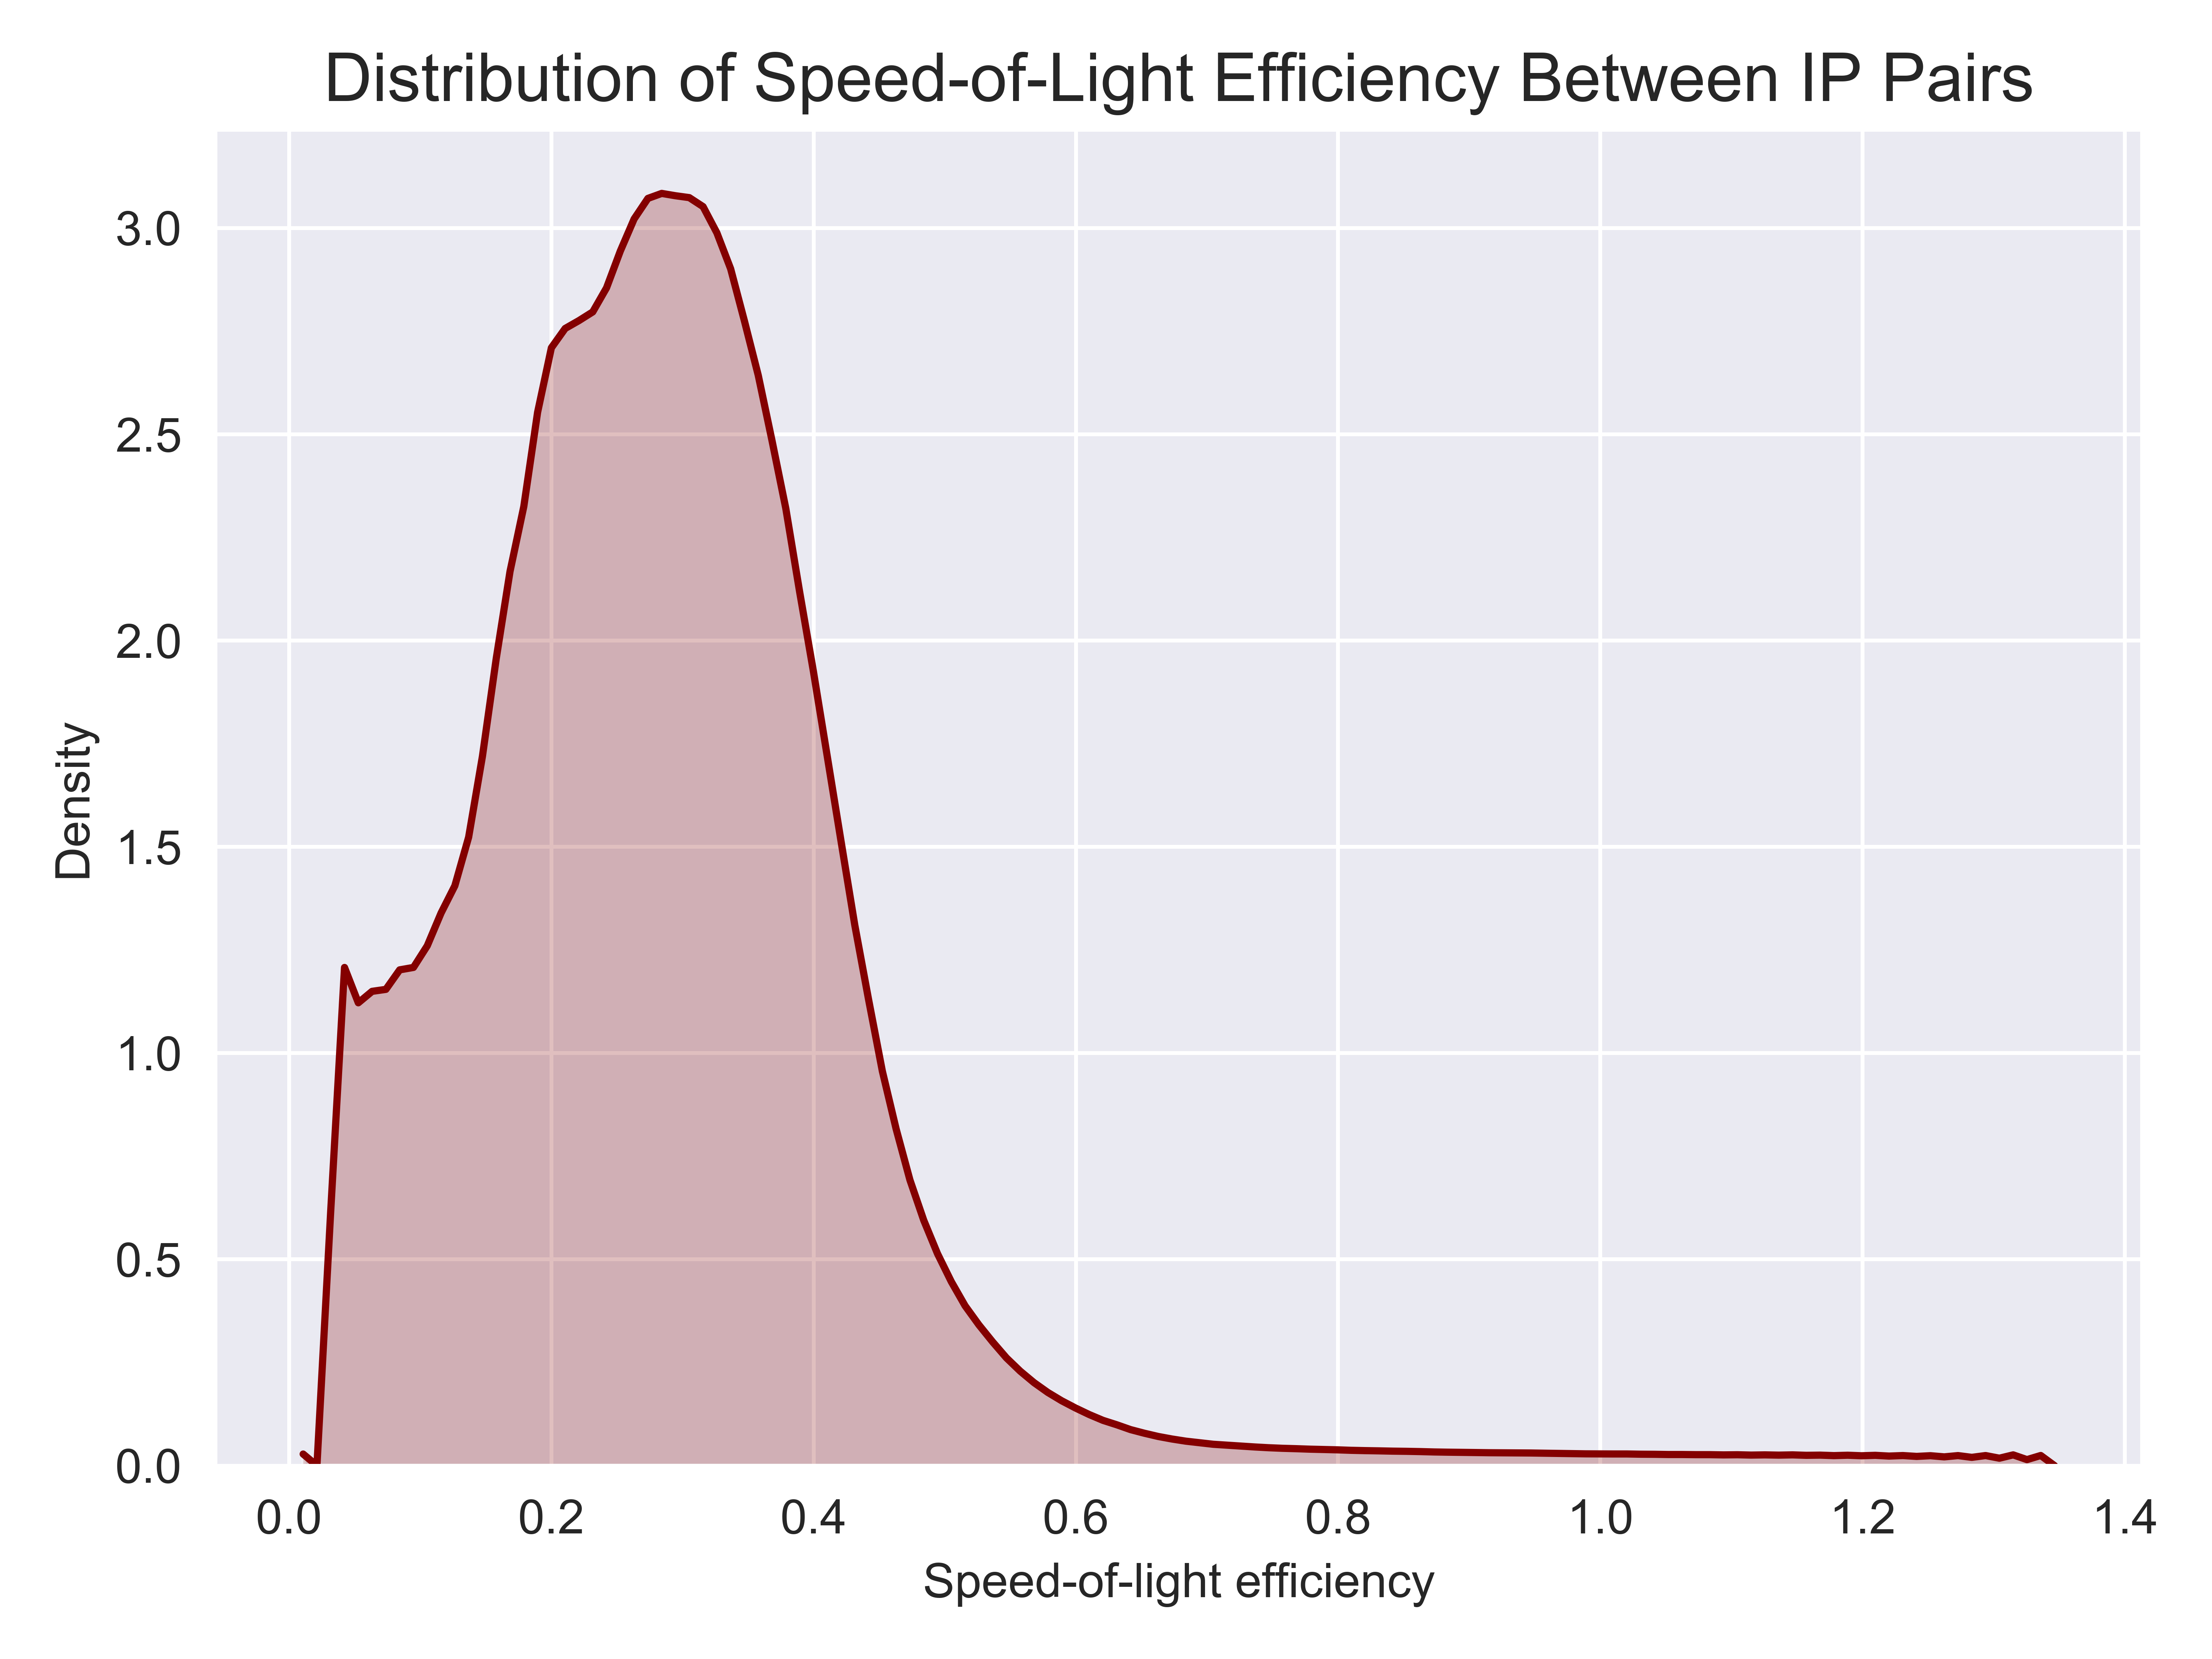
\includegraphics[width=0.75\textwidth]{caida/frac_c_efficiency_distribution.png}
    \caption{Distribution of speed-of-light efficiencies}
    \label{fig:speed_of_light_efficiency_distribution}
\end{figure}

\subsection{Mapping}

The most immediate way of mapping a set of points on a coordinate plane with values attached to each of them is a a simple
scatterplot, but with massive amounts of unevenly distributed data it becomes tough to visualize and draw conclusions. For example, in \autoref{fig:caida_scatterplot} we see point for \textit{every single data point} in the \caida and \ripe Atlas data set that was collected and analyzed.

\begin{figure}[H]
    \centering
    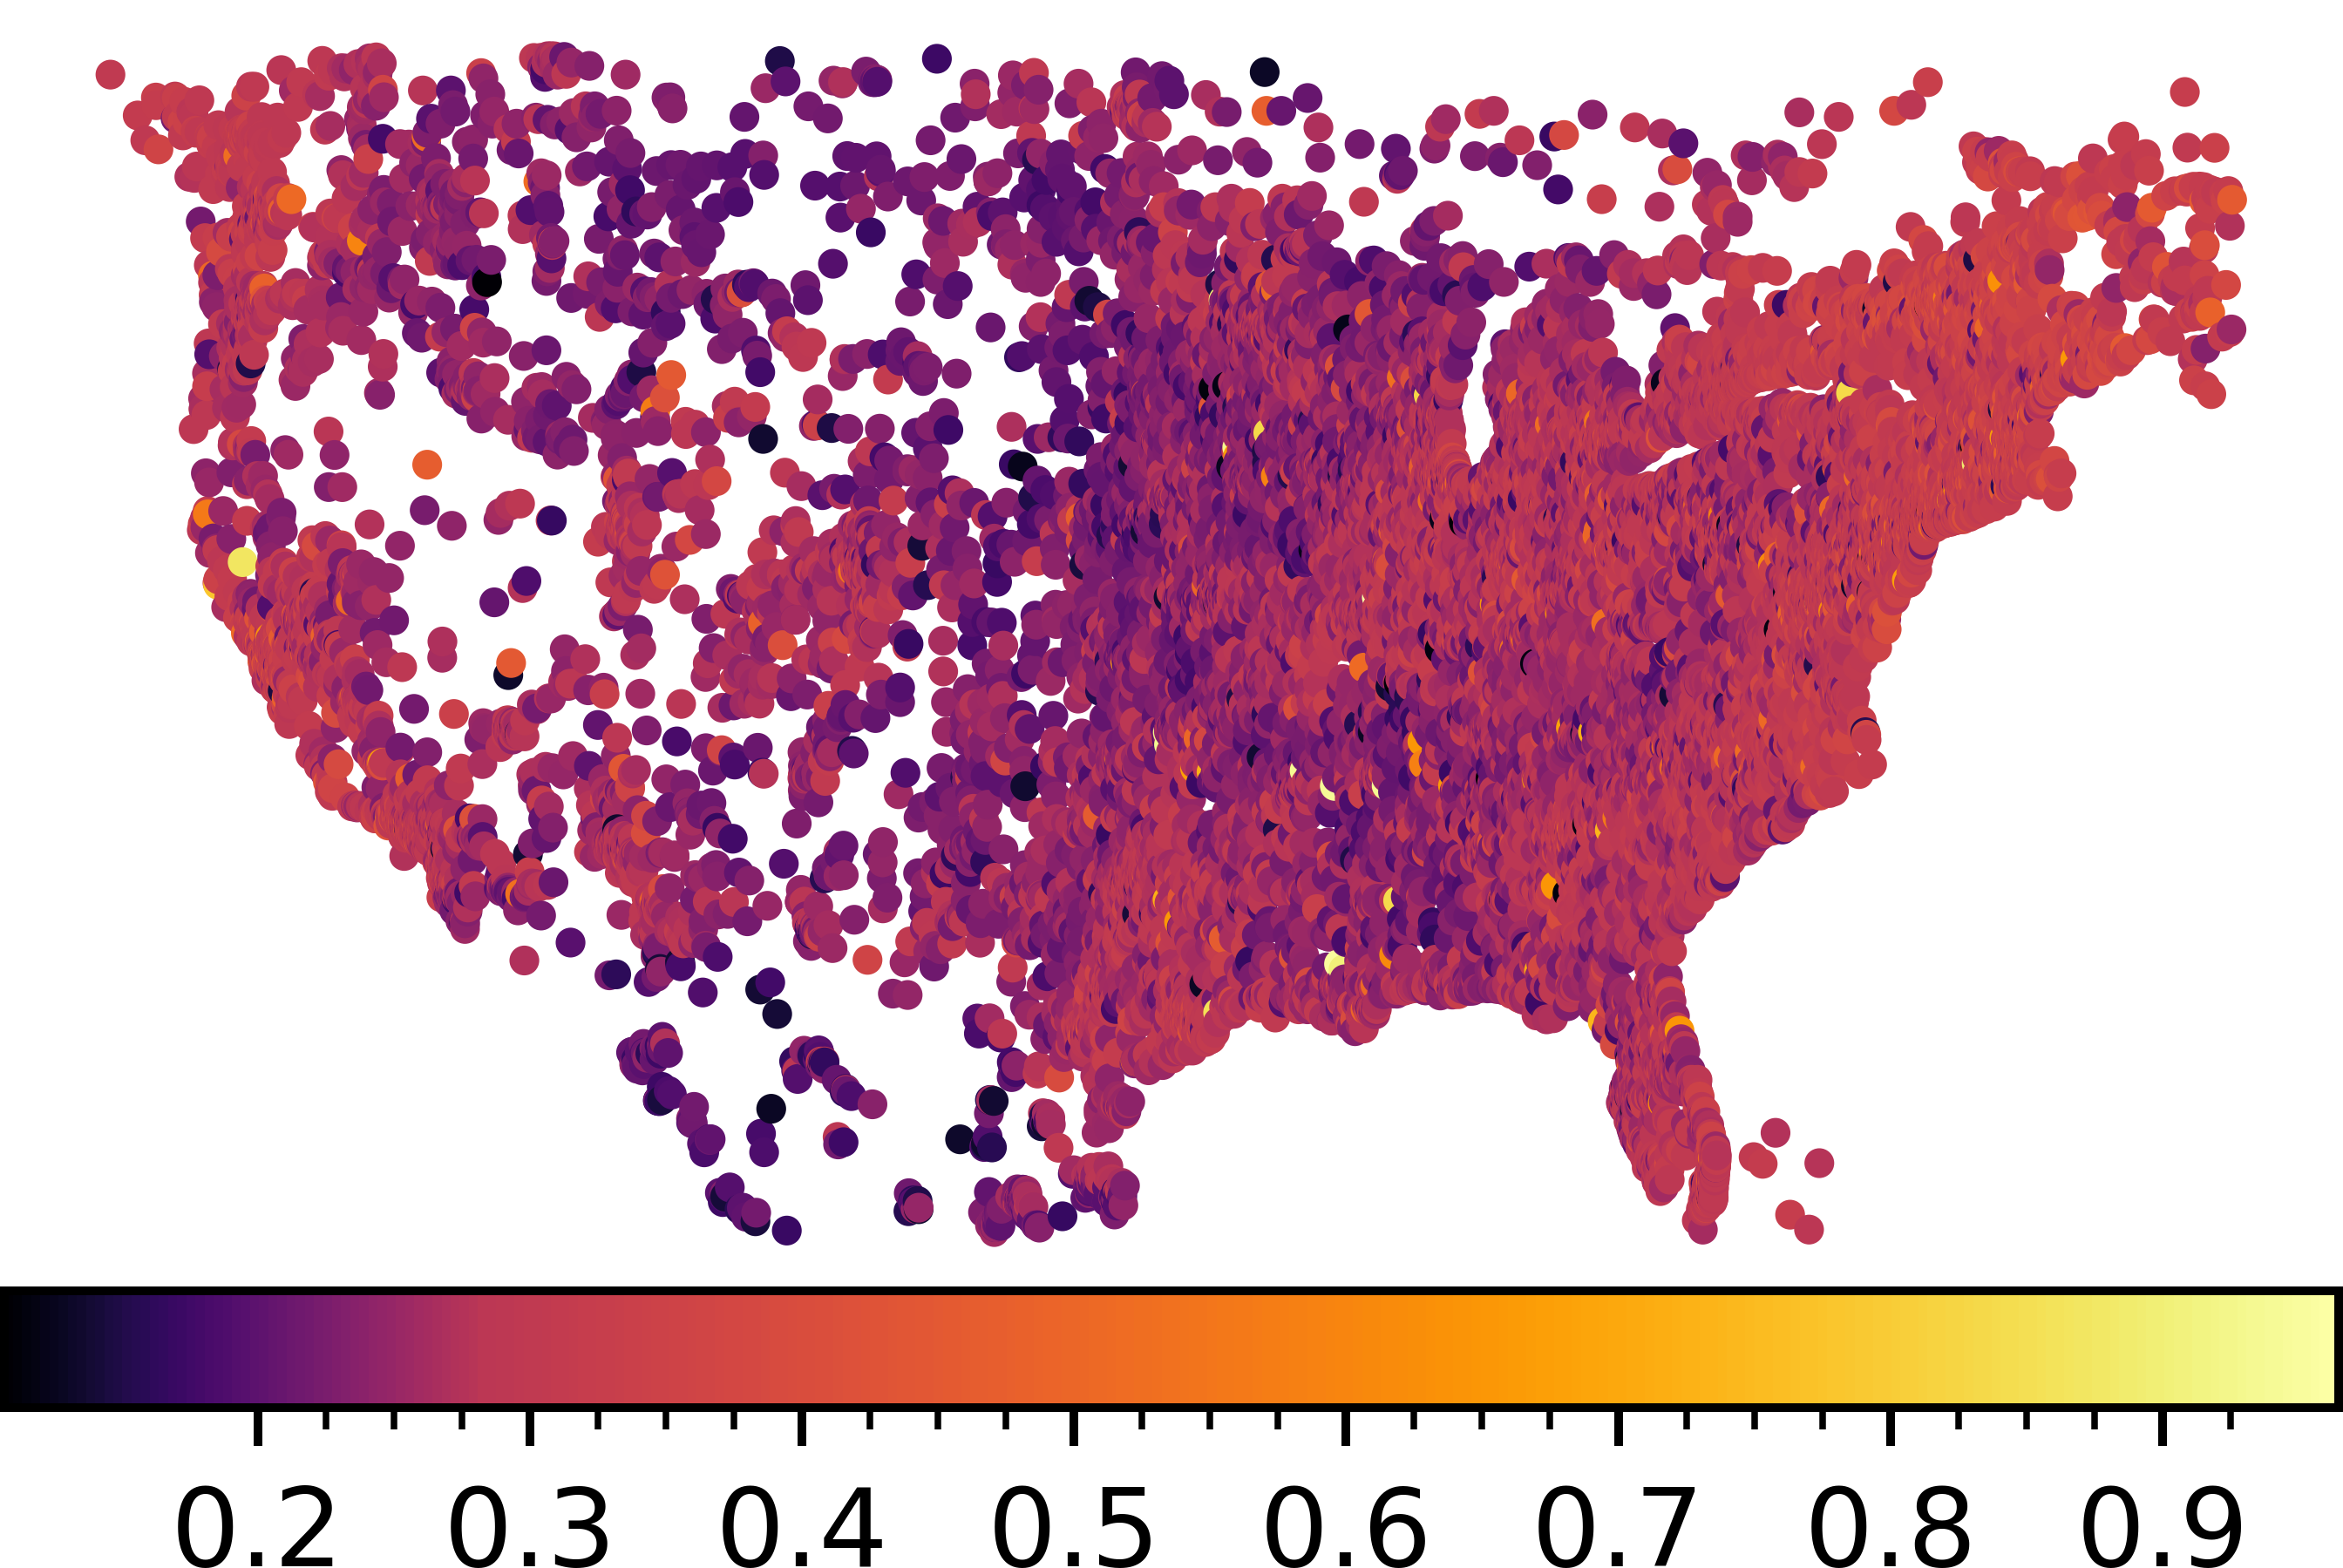
\includegraphics[width=0.75\textwidth]{caida/scatterplot.png}
    \caption{Scatterplot of CAIDA data, normalized and colored by speed of light efficiency}
    \label{fig:caida_scatterplot}
\end{figure}

Some simple relationships can be inferred with moderate difficulty, like better internet connections near the coast or major cities, but otherwise this map is truly only good at confirming that geolocation of IP addresses works. Many areas simply don't have measurements either, and those that appear covered look that way because the dots for each measurement were inflated for visual effect. If they were more accurately represented to-scale as single pixels, the map would be very sparse.

To solve this problem the map needed some interpolation to fill in the gaps and make the data easier to understand. Ideally someone looking at the map should be able to point to a spot on the map and get an estimated value for connectivity at that location, even if there wasn't a measurement at precisely that location. Different methods of interpolation are available, the simplest of which is nearest-neighbor interpolation.

\begin{figure}[H]
    \centering
    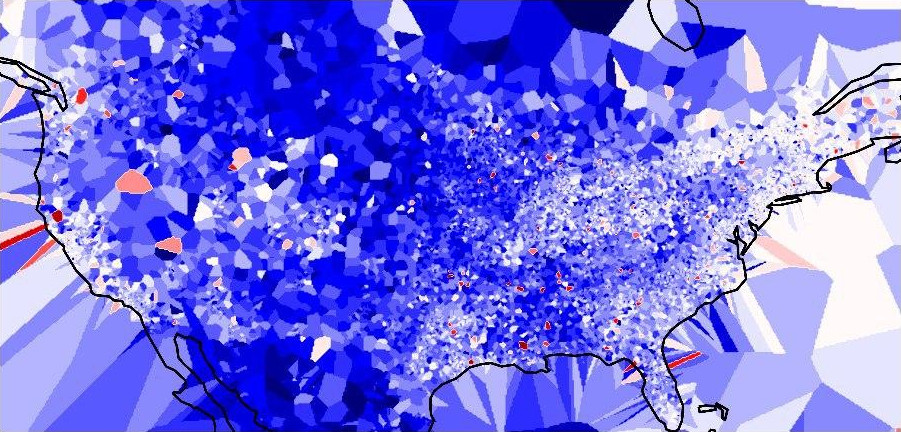
\includegraphics[width=0.75\textwidth]{caida/nearest_neighbor.jpg}
    \caption{Nearest-neighbor (Voronoi) diagram of speed-of-light efficiency data, divergent colormap}
    \label{fig:caida_nearest_neighbor}
\end{figure}

\autoref{fig:caida_nearest_neighbor} shows a nearest-neighbor plot, otherwise known as a Voronoi diagram \cite{Malhotra2017LoveNeighbors}, of the \caida and \ripe Atlas data combined, generated with Python matplotlib and scikit-learn. The colormap is a divergent linear colormap, where blue is worse-than-average and red is better-than-average efficiency. This does an arguably better job of presenting the data, but it's visually noisy and suffers from expanded influence of points in small areas. For instance, consider the large red splotch in Utah, which corresponds to Salt Lake City. While it's likely accurate that the city has far better internet connectivity than its desert surroundings, it is likely inaccurate to say that the areas within the few hundred mile radius shown on the map have the same level of connectivity.

\FloatBarrier
